%% History:
% Pavel Tvrdik (26.12.2004)
%  + initial version for PhD Report
%
% Daniel Sykora (27.01.2005)
%
% Michal Valenta (3.12.2008)
% rada zmen ve formatovani (diky M. Duškovi, J. Holubovi a J. Žďárkovi)
% sjednoceni zdrojoveho kodu pro anglickou, ceskou, bakalarskou a diplomovou praci

% One-page layout: (proof-)reading on display
%%%% \documentclass[11pt,oneside,a4paper]{book}
% Two-page layout: final printing
\documentclass[11pt,twoside,a4paper]{book}   
\renewcommand{\baselinestretch}{1.0} 
%=-=-=-=-=-=-=-=-=-=-=-=--=%
% The user of this template may find useful to have an alternative to these 
% officially suggested packages:
\usepackage[czech, english]{babel}
\addto\captionsczech{\renewcommand{\bibname}{Reference}}
\usepackage[T1]{fontenc} % pouzije EC fonty 
% pripadne pisete-li cesky, pak lze zkusit take:
% \usepackage[OT1]{fontenc} 
\usepackage[utf8]{inputenc}
%=-=-=-=-=-=-=-=-=-=-=-=--=%
% In case of problems with PDF fonts, one may try to uncomment this line:
%\usepackage{lmodern}
%=-=-=-=-=-=-=-=-=-=-=-=--=%
%=-=-=-=-=-=-=-=-=-=-=-=--=%
% Depending on your particular TeX distribution and version of conversion tools 
% (dvips/dvipdf/ps2pdf), some (advanced | desperate) users may prefer to use 
% different settings.
% Please uncomment the following style and use your CSLaTeX (cslatex/pdfcslatex) 
% to process your work. Note however, this file is in UTF-8 and a conversion to 
% your native encoding may be required. Some settings below depend on babel 
% macros and should also be modified. See \selectlanguage \iflanguage.
%\usepackage{czech}  %%%%%\usepackage[T1]{czech} %%%%[IL2] [T1] [OT1]
%=-=-=-=-=-=-=-=-=-=-=-=--=%

%%%%%%%%%%%%%%%%%%%%%%%%%%%%%%%%%%%%%%%
% Styles required in your work follow %
%%%%%%%%%%%%%%%%%%%%%%%%%%%%%%%%%%%%%%%
\usepackage{graphicx}
%\usepackage{indentfirst} %1. odstavec jako v cestine.

\usepackage{k336_thesis_macros} % specialni makra pro formatovani DP a BP 
 % muzete si vytvorit i sva vlastni v souboru k336_thesis_macros.sty
 % najdete  radu jednoduchych definic, ktere zde ani nejsou pouzity
 % napriklad: 
 % \newcommand{\bfig}{\begin{figure}\begin{center}}
 % \newcommand{\efig}{\end{center}\end{figure}}
 % umoznuje pouzit prikaz \bfig namisto \begin{figure}\begin{center} atd.

\usepackage{enumerate}
\usepackage{listings}
% \lstset{language=java,
% numberstyle=\footnotesize,
% basicstyle=\footnotesize,
% basicstyle=\ttfamily,
% numbers=left,
% stepnumber=1,
% frame=shadowbox,
% breaklines=true}

\lstset{
           basicstyle=\scriptsize\ttfamily,
           numberstyle=\footnotesize,
           numbers=left,
           stepnumber=1,
%            frame=shadowbox,
%            breaklines=true
          }

\usepackage{eurosym}
\usepackage{array}
\usepackage[export]{adjustbox}
\usepackage[usenames, dvipsnames]{xcolor}

\lstnewenvironment{code}[1][]%
  {\noindent\minipage{\linewidth}\medskip 
   \lstset{basicstyle=\ttfamily\footnotesize,frame=single,#1}}
  {\endminipage}
  


%%%%%%%%%%%%%%%%%%%%%%%%%%%%%%%%%%%%%
% Zvolte jednu z moznosti 
% Choose one of the following options
%%%%%%%%%%%%%%%%%%%%%%%%%%%%%%%%%%%%%
\newcommand\TypeOfWork{Diplomová práce} \typeout{Diplomova prace}
% \newcommand\TypeOfWork{Master's Thesis}   \typeout{Master's Thesis} 
% \newcommand\TypeOfWork{Bakalářská práce}  \typeout{Bakalarska prace}
% \newcommand\TypeOfWork{Bachelor's Project}  \typeout{Bachelor's Project}


%%%%%%%%%%%%%%%%%%%%%%%%%%%%%%%%%%%%%
% Zvolte jednu z moznosti 
% Choose one of the following options
%%%%%%%%%%%%%%%%%%%%%%%%%%%%%%%%%%%%%
% nabidky jsou z: http://www.fel.cvut.cz/cz/education/bk/prehled.html

%\newcommand\StudProgram{Elektrotechnika a informatika, dobíhající, Bakalářský}
%\newcommand\StudProgram{Elektrotechnika a informatika, dobíhající, Magisterský}
% \newcommand\StudProgram{Elektrotechnika a informatika, strukturovaný, Bakalářský}
 \newcommand\StudProgram{Otevřená informatika, strukturovaný, Navazující magisterský}
% \newcommand\StudProgram{Softwarové technologie a management, Bakalářský}
% English study:
% \newcommand\StudProgram{Electrical Engineering and Information Technology}  % bachelor programe
% \newcommand\StudProgram{Electrical Engineering and Information Technology}  %master program


%%%%%%%%%%%%%%%%%%%%%%%%%%%%%%%%%%%%%
% Zvolte jednu z moznosti 
% Choose one of the following options
%%%%%%%%%%%%%%%%%%%%%%%%%%%%%%%%%%%%%
% nabidky jsou z: http://www.fel.cvut.cz/cz/education/bk/prehled.html

%\newcommand\StudBranch{Výpočetní technika}   % pro program EaI bak. (dobihajici i strukt.)
%\newcommand\StudBranch{Výpočetní technika}   % pro prgoram EaI mag. (dobihajici i strukt.) 
\newcommand\StudBranch{Softwarové inženýrství}            %pro STM
%\newcommand\StudBranch{Web a multimedia}                  % pro STM
%\newcommand\StudBranch{Computer Engineering}              % bachelor programe
%\newcommand\StudBranch{Computer Science and Engineering}  % master programe


%%%%%%%%%%%%%%%%%%%%%%%%%%%%%%%%%%%%%%%%%%%%
% Vyplnte nazev prace, autora a vedouciho
% Set up Work Title, Author and Supervisor
%%%%%%%%%%%%%%%%%%%%%%%%%%%%%%%%%%%%%%%%%%%%

\newcommand\WorkTitle{Nástroj pro generování dokumentace vzdálených rozhraní
(API) webových služeb aplikací Java Enterprise Edition}
\newcommand\FirstandFamilyName{Bc.
Tomáš Jiříček} \newcommand\Supervisor{Ing. Tomáš Černý, MSc.}


% Pouzijete-li pdflatex, tak je prijemne, kdyz bude mit vase prace
% funkcni odkazy i v pdf formatu
\usepackage[
pdftitle={\WorkTitle},
pdfauthor={\FirstandFamilyName},
bookmarks=true,
colorlinks=true,
breaklinks=true,
urlcolor=red,
citecolor=blue,
linkcolor=blue,
unicode=true,
% hidelinks
]
{hyperref}



% Extension posted by Petr Dlouhy in order for better sources reference ( \cite{} command) especially in Czech.
% April 2010
% See comment over \thebibliography command for details.

\usepackage[square, numbers]{natbib}             % sazba pouzite literatury
%\usepackage{url}
%\DeclareUrlCommand\url{\def\UrlLeft{<}\def\UrlRight{>}\urlstyle{tt}}  %rm/sf/tt
%\renewcommand{\emph}[1]{\textsl{#1}}    % melo by byt kurziva nebo sklonene,
\let\oldUrl\url
\renewcommand\url[1]{<\texttt{\oldUrl{#1}}>}
\urlstyle{same}
\begin{document}

%%%%%%%%%%%%%%%%%%%%%%%%%%%%%%%%%%%%%
% Zvolte jednu z moznosti 
% Choose one of the following options
%%%%%%%%%%%%%%%%%%%%%%%%%%%%%%%%%%%%%
\selectlanguage{czech}
%\selectlanguage{english} 

% prikaz \typeout vypise vyse uvedena nastaveni v prikazovem okne
% pro pohodlne ladeni prace


\iflanguage{czech}{
	 \typeout{************************************************}
	 \typeout{Zvoleny jazyk: cestina}
	 \typeout{Typ prace: \TypeOfWork}
	 \typeout{Studijni program: \StudProgram}
	 \typeout{Obor: \StudBranch}
	 \typeout{Jmeno: \FirstandFamilyName}
	 \typeout{Nazev prace: \WorkTitle}
	 \typeout{Vedouci prace: \Supervisor}
	 \typeout{***************************************************}
	 \newcommand\Department{Katedra počítačů}
	 \newcommand\Faculty{Fakulta elektrotechnická}
	 \newcommand\University{České vysoké učení technické v~Praze}
	 \newcommand\labelSupervisor{Vedoucí práce}
	 \newcommand\labelStudProgram{Studijní program}
	 \newcommand\labelStudBranch{Obor}
}{
	 \typeout{************************************************}
	 \typeout{Language: english}
	 \typeout{Type of Work: \TypeOfWork}
	 \typeout{Study Program: \StudProgram}
	 \typeout{Study Branch: \StudBranch}
	 \typeout{Author: \FirstandFamilyName}
	 \typeout{Title: \WorkTitle}
	 \typeout{Supervisor: \Supervisor}
	 \typeout{***************************************************}
	 \newcommand\Department{Department of Computer Science and Engineering}
	 \newcommand\Faculty{Faculty of Electrical Engineering}
	 \newcommand\University{Czech Technical University in Prague}
	 \newcommand\labelSupervisor{Supervisor}
	 \newcommand\labelStudProgram{Study Programme} 
	 \newcommand\labelStudBranch{Field of Study}
}




%%%%%%%%%%%%%%%%%%%%%%%%%%    Poznamky ke kompletaci prace
% Nasledujici pasaz uzavrenou v {} ve sve praci samozrejme 
% zakomentujte nebo odstrante. 
% Ve vysledne svazane praci bude nahrazena skutecnym 
% oficialnim zadanim vasi prace.
{
\pagenumbering{roman} \cleardoublepage \thispagestyle{empty}
\chapter*{Na tomto místě bude oficiální zadání vaší práce}
\begin{itemize}
\item Toto zadání je podepsané děkanem a vedoucím katedry,
\item musíte si ho vyzvednout na studiijním oddělení Katedry počítačů na Karlově náměstí,
\item v~jedné odevzdané práci bude originál tohoto zadání (originál zůstává po obhajobě na katedře),
\item ve druhé bude na stejném místě neověřená kopie tohoto dokumentu (tato se vám vrátí po obhajobě).
\end{itemize}
\newpage
}

%%%%%%%%%%%%%%%%%%%%%%%%%%    Titulni stranka / Title page 

\coverpagestarts

%%%%%%%%%%%%%%%%%%%%%%%%%%%    Podekovani / Acknowledgements 

\acknowledgements
\noindent
Velmi rád bych poděkoval svým rodičům za podporu při studiích a důvěru ve mě.
Velký dík posílám také přítelkyni Veronice. 

Dále bych rád poděkoval Mgr.
Ivu Bekovi a Ing. Tomáši Černému, MSc. za připomínky a odborné rady při tvorbě
této práce.


%%%%%%%%%%%%%%%%%%%%%%%%%%%   Prohlaseni / Declaration 

\declaration{V~Praze dne 10.\,5.\,2015}
%\declaration{In Kořenovice nad Bečvárkou on May 15, 2008}


%%%%%%%%%%%%%%%%%%%%%%%%%%%%    Abstract 
 
\abstractpage

With the increasing number of software products, which have a need to be
integrated in between themselves, a big pressure developed with interface
unification. Therefore a row of protocols and technologies was developed, which
brings rules into system integration and aproaches, which designate how the
remote communication between system should work and how to create providers and
clients of such interfaces.
If there is a required documentation for an interface, which enables the
consumer to obtain all needed information about the interface, it is fairly easy
to realize the integration. In reversed case incomplete, nonactual or otherwise
insufficient documentation can lead to growth of needed funds for the
realization of integration.

The aim of the thesis is to analyze the requirements of the documentation and to
develop a tool for automatic generation of actual documentation of remote
interfaces. With the usage of the tool there will be a decrease of needed funds
for the development of the documentation and for the realization of the system
integration.

% Prace v cestine musi krome abstraktu v anglictine obsahovat i
% abstrakt v cestine.
\vglue35mm

\noindent{\Huge \textbf{Abstrakt}}
\vskip 2.75\baselineskip
% \noindent
S~narůstajícím počtem softwarových produktů, které mají potřebu být mezi sebou vzájemně
integrovány vznikl velký tlak na unifikaci rozhraní. Byla proto vytvořena řada protokolů a
technologií, které přinášejí do systémové integrace pravidla a postupy určující,
jak probíhá vzdálená komunikace mezi systémy a jak tvořit poskytovatele a klienty takových rozhraní.
Pokud existuje k~vystavenému rozhraní odpovídající dokumentace, která umožní
konzumentovi poskytnout všechny potřebné informace o~rozhraní, lze poměrně rychle a
jednoduše provést integraci. V~opačném případě nekompletní, neaktuální či jinak
nedostačující dokumentace může způsobit nárust nákladů na realizování integrace.

Cílem práce je analyzovat požadavky dokumentace a vytvořit nástroj pro automatické
generování aktuální dokumentace vzdálených rozhraní. S~využitím nástroje dojde ke snížení
nákladů potřebných pro tvorbu dokumentace a tím i realizaci systémové integrace.


%%%%%%%%%%%%%%%%%%%%%%%%%%%%%%%%  Obsah / Table of Contents 

\tableofcontents
\addtocontents{toc}{\setcounter{tocdepth}{2}} 


%%%%%%%%%%%%%%%%%%%%%%%%%%%%%%%  Seznam obrazku / List of Figures 

\listoffigures


%%%%%%%%%%%%%%%%%%%%%%%%%%%%%%%  Seznam tabulek / List of Tables

\listoftables

\lstlistoflistings 


%**************************************************************

\mainbodystarts
% horizontalní mezera mezi dvema odstavci
%\parskip=5pt
%11.12.2008 parskip + tolerance
\normalfont
\parskip=0.2\baselineskip plus 0.2\baselineskip minus 0.1\baselineskip

% Odsazeni prvniho radku odstavce resi class book (neaplikuje se na prvni 
% odstavce kapitol, sekci, podsekci atd.) Viz usepackage{indentfirst}.
% Chcete-li selektivne zamezit odsazeni 1. radku nektereho odstavce,
% pouzijte prikaz \noindent.

%**************************************************************

% Pro snadnejsi praci s vetsimi texty je rozumne tyto rozdelit
% do samostatnych souboru nejlepe dle kapitol a tyto potom vkladat
% pomoci prikazu \include{jmeno_souboru.tex} nebo \include{jmeno_souboru}.
% Napr.:
% \include{1_uvod}
% \include{2_teorie}
% atd...

%*****************************************************************************
% \chapter{Úvod}
% \section*{}
Systémová integrace je velmi často skloňovaný pojem. Drtivá většina systémů v dnešní době
není bez integrace schopna fungovat. Schopnost integrace s jinými systémy je žádoucí,
protože čím více se umí software integrovat, tím je flexibilnější. Integrace znamená spojení
menších komponent do vetšího celku. Takový celek potom dokáže efektivně pracovat pomocí
definovaných pravidel pro komunikaci mezi subsytémy. Integraci lze vytvořit na různých
systémových vrstvách.

První počátky integrace sahají do roku 1980, kdy vznikla myšlenka tzv. digitální výroby, která
byla aplikována v továrnách. V devadesátých letech společnosti nakupovaly softwarová řešení
jako je SAP, Oracle ERP, Siebel a další. Tato řešení fungovala dobře jako samostatný
software, vytvořily se kolem nich takzvané informační ostrovy. Ve většině případů každé
řešení produkovalo redundantní data. Ve výsledku při vzniklé změně dat musely být ručně
změněny i v ostatních systémech. Takové řešení bylo těžkopádné a musela přijít změna. Tyto
problémy daly vzniknout rozmachu integrace mezi systémy.

Komunikace mezi komponentami byla často platformově závislá a používaly se pro ni
proprietární protokoly. Postupem času, jak šly informační technologie dopředu a sílil tlak na
vznik technologií umožňujících platformovou nezávislost s otevřenými protokoly pro
komunikaci, jsme ve stavu, kdy máme technologie a standardizované protokoly. S jejich
pomocí vznikají unifikovaná rozhraní systémů, která zjednodušují realizování integrace mezi
softwarovými komponentami.

Protokoly definují jak probíhá komunikace, technologie definují jak vytvářet rozhraní a
klienty k nim, opomíjí se však tvorba, obsah a umístění dokumentace. Přestože poskytovatelé
rozhraní používají jednotné protokoly a technologie, dokumentaci má každý trochu jinou.
Momentálně se můžeme setkat nejčastěji s dokumentací v HTML, dokumentech
kancelářských balíků či PDF dokumentech. Taková dokumentace je tvořena ručně a má řadu
nevýhod. Při její tvorbě může být zanesena chyba, dokumentace nemusí být aktuální a nemusí
odpovídat popisovanému rozhraní. Dále usí existovat člověk, který bude za dokumentaci
zodpovědný. Provádět integraci se systémem mající neodpovídající dokumentaci může
prodloužit dobu integrace a tím vzrostou náklady.

Cílem diplomové práce je navrhnout, implementovat a otestovat nástroj pro automatické
generování dokumentace vzdálených rozhraní. Nástroj by měl odstranit problémy s tvorbou
dokumentace, protože proces její tvorby nebude zahrnovat lidský element a bude zajištěno,
aby se dokumentace aktualizovala vždy se změnou rozhraní. 

\end{document}
\chapter{Úvod} 
% \section*{}
Systémová integrace je velmi často skloňovaný pojem. Drtivá většina systémů v~dnešní době
není bez integrace schopna fungovat. Schopnost integrace s~jinými systémy je žádoucí,
protože čím více se umí software integrovat, tím je flexibilnější. Integrace znamená spojení
menších komponent do vetšího celku. Takový celek potom dokáže efektivně pracovat pomocí
definovaných pravidel pro komunikaci mezi subsytémy. Integraci lze vytvořit na různých
systémových vrstvách.

První počátky integrace sahají do roku 1980, kdy vznikla myšlenka tzv. digitální výroby, která
byla aplikována v~továrnách. V~devadesátých letech společnosti nakupovaly softwarová řešení
jako je SAP, Oracle ERP, Siebel a další. Tato řešení fungovala dobře jako samostatný
software, vytvořily se kolem nich takzvané informační ostrovy. Ve většině případů každé
řešení produkovalo redundantní data. Ve výsledku, při vzniklé změně dat, musela
být redundantní data ručně změněna i v~ostatních systémech. Takové řešení bylo
těžkopádné a musela přijít změna. Tyto problémy daly vzniknout rozmachu integrace mezi systémy.

Komunikace mezi komponentami byla často platformově závislá a používaly se pro ni
proprietární protokoly. Postupem času, jak šly informační technologie dopředu a sílil tlak na
vznik technologií umožňujících platformovou nezávislost s~otevřenými protokoly pro
komunikaci, jsme se dostali do stavu, kdy máme technologie a standardizované
protokoly.
S~jejich pomocí vznikají unifikovaná rozhraní systémů, která zjednodušují realizování integrace mezi
softwarovými komponentami.

Protokoly definují, jak probíhá komunikace a technologie definují, jak vytvářet
rozhraní a klienty k~nim, opomíjí se však tvorba, obsah a umístění dokumentace. Přestože poskytovatelé
rozhraní používají jednotné protokoly a technologie, dokumentaci má každý mírně
odlišnou.
Momentálně se můžeme setkat nejčastěji s~dokumentací v~HTML, dokumentech
kancelářských balíků či PDF dokumentech. Taková dokumentace je tvořena ručně a má řadu
nevýhod. Při její tvorbě může být zanesena chyba, dokumentace nemusí být aktuální a nemusí
odpovídat popisovanému rozhraní. Dále musí existovat člověk, který bude za
dokumentaci zodpovědný. Provádět integraci se systémem mající neodpovídající dokumentaci může
prodloužit dobu integrace a tím vzrostou náklady.

Cílem diplomové práce je navrhnout, implementovat a otestovat nástroj pro automatické
generování dokumentace vzdálených rozhraní. Nástroj by měl odstranit problémy s~tvorbou
dokumentace, protože proces její tvorby nebude zahrnovat lidský element a bude zajištěno,
aby se dokumentace aktualizovala vždy se změnou rozhraní.

\chapter{Analýza}
\section{Specifikace technologií pro vzdálená rozhraní}
Způsobů, jak na platformě Java EE vzdáleně komunikovat mezi systémy přes
počítačovou síť, je několik. V~současné době se pro integraci nejvíce používají
webové služby založené na SOAP zprávách a také služby založené na architektonickém stylu
REST. Dalšími způsoby vzdálené komunikace jsou například JMS, RMI nebo CORBA.
Tato práce se zabývá prvními dvěmi zmíněnými.

\subsection{SOAP-based webová služba}

SOAP-based webová služba \cite{Kalin13} je způsob komunikace mezi počítači.
Komunikace, struktura zpráv, popis služeb a registr těchto služeb jsou řízeny otevřenými protokoly, které se
neustále vyvýjejí. Díky otevřenosti jsou SOAP-based webové služby platformově
nezávislé. Technologie užívané v~SOAP-based webových službách v~této práci
podléhají následujícím verzím:

\begin{itemize}
 \item XML 1.0
  \item WSDL 1.1
  \item SOAP 1.2
\end{itemize}

První verze protokolu SOAP pochází z~roku 1999 od společností Microsoft, IBM a
dalších. Pro SOAP-based webové služby jsou definovány čtyři hlavní protokoly.

\subsubsection{Transportní protokol (Transport Protocol)}

Přes transportní protokol jsou posílány zprávy po síti. Jako transportní
protokol se nejčastěji využívá HTTP, SMTP a FTP. V~prostředí jazyka Java lze
použít i JMS, což je API pro posílání zpráv. Toto API nemá pevně definován WP,
který je zodpovědný za přenos zpráv, ale je možné si zvolit mezi různými
protokoly od různých implementací JMS. JMS nařizuje, aby různé implementace
dokázaly mezi sebou komunikovat. Praxe však ukazuje, že ne všechny jsou mezi
sebou plně kompatibilní.

\subsubsection{Protokol zpráv (Messaging Protocol)}

\begin{figure}[h]
\begin{center}
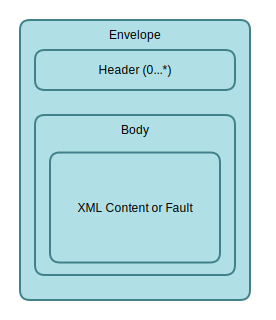
\includegraphics[width=7cm]{images-pdf/soap.pdf} 
\caption{SOAP zpráva}
\label{fig:soap-zprava}
\end{center}
\end{figure}

Protokol zpráv je zodpovědný za zakódování a dekódování zprávy do, resp.
z~XML-based formátu. Nejčastěji se užívá protokol
SOAP \cite{OraSOAP} \cite{WikiSOAP}. Na \ref{fig:soap-zprava} je vyobrazena
struktura SOAP zprávy. SOAP protokol udává, jak bude vypadat přenášená zpráva,
která se skládá ze čtyř hlavních částí:

\begin{itemize}
\item \textbf{\textit{Envelope}} – kořenový element SOAP zprávy, který je povinný a definuje, že jeho
obsahem je SOAP zpráva.

\item \textbf{\textit{Header}} – volitelný element, který se používá pro přidání
nové funkcionality a vlastností, jakou může být například autentizace. Ve zprávě je povoleno použít více
těchto elementů. Pokud je header ve zprávě přítomen, musí být umístěn jako první
přímý potomek elementu envelope.
 
\item \textbf{\textit{Body}} – povinný element, který obsahuje přenášená
data nazývána „payload“. Body musí být uvnitř elementu envelope a následuje až
za elementy header. Sémantika obsahu v~elementu body je definována v~XML Schema.

\item \textbf{\textit{Fault}} – tento element je umístěn v~elementu body.
Ve zprávě se objevuje, pokud je nutné poslat informaci o~vzniklé chybě. Fault má definováno, jak má informace
o~chybě vypadat a obsahuje následující subelementy:

\begin{itemize}
  \item \textit{faultCode},
  \item \textit{faultString},
  \item \textit{faultActor},
  \item \textit{detail}.
\end{itemize}
\end{itemize}

\subsubsection{Protokol popisující službu (Description Protocol)}

\begin{figure}[h]
\begin{center}
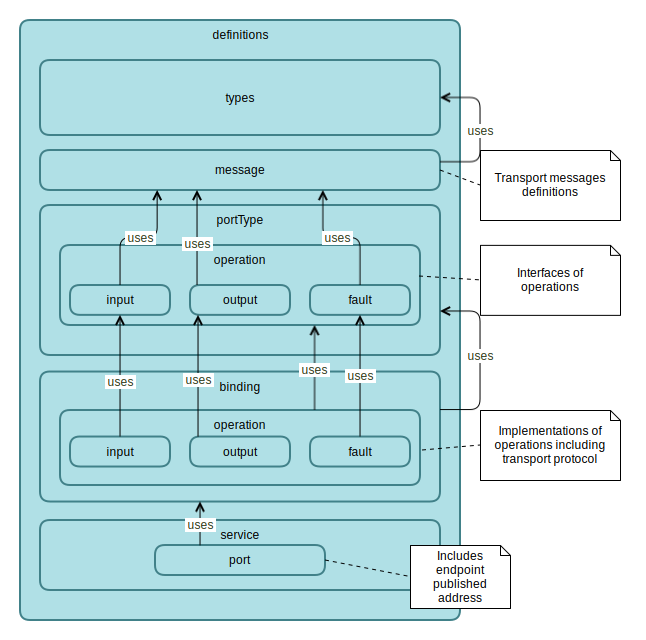
\includegraphics[width=12cm]{images-pdf/wsdl.pdf} 
\caption{Struktura WSDL}
\label{fig:struktura-wsdl}
\end{center}
\end{figure}

Tento protokol popisuje veřejné rozhraní dané SOAP-based webové služby. Typicky
se používá WSDL, což je XML-based protokol. WSDL definuje, jak ke službě
přistupovat a jaké metody můžeme na službě volat. V~tomto protokolu jsou dále
zaneseny například informace, jaké má metoda parametry, jaké návratové hodnoty a
jaké mohou nastat faulty při volání metody.

Kořenový element WSDL dokumentu se jmenuje \textit{definitions}. Schéma elementu
je na vidět \ref{fig:struktura-wsdl}.
Definitons formuluje název webové služby a deklaruje jmenné prostory, takzvané
„namespace“. Uvnitř elementu definitions je několik přímých potomků:

\begin{itemize}
  \item \textbf{\textit{Types}} - element obsahující všechny datové typy,
  které se mohou přenášet. Datové typy jsou zapsány v~XML Schema.

  \item \textbf{\textit{Message}} – značí abstrakci přenášené zprávy.
  Těchto elementů bývá zpravidla více, protože pro jednu metodu, která má mít
  vstup, výstup a fault, musí existovat tři tyto
elementy. Části elementu message se budou skládat z~datových typů definovaných
v~elementu types.

  \item \textbf{\textit{PortType}} – jedná se o~abstraktní množinu operací
k~jednomu nebo více endpointům\footnote{Rozhraní publikované služby}, které
  mohou být volány.
  Těmto operacím se potom v~elementu \textit{binding} nastavuje transportní protokol.

  \begin{itemize}
    \item \textit{Operation} - přímý potomek elementu portType,
    který lze přirovnat k~metodě v~klasických programovacích jazycích, jako je
    například Java či C. V~tomto elementu je definováno jméno metody, input message, output message a fault.
Části input, output a fault se odkazují na definice v~elementech message.

  \end{itemize}
  \item \textbf{\textit{Binding}} – tento element definuje pro každý
  portType konkrétní datové typy, operace a protokol.

  \item \textbf{\textit{Service}} - poslední přímý potomek kořenového
  elementu. Uvnitř něj je definován seznam endpointů. Binding služby je zde
  mapován na \textit{port}.

  \begin{itemize}
    \item \textit{Port} - přímý potomek elementu service. Port je
    kombinací bindingu a síťové adresy, na které je služba dostupná.

  \end{itemize}
\end{itemize}

\subsubsection{Protokol pro objevování služeb (Discovery Protocol)}
Protokol pro objevování služeb je XML-based registr, díky němuž mohou být po celém
internetu shromažďovány informace o~webových službách. Umožňuje zaregistrování webové
služby a jejich procházení v~daném registru, který nazýváme UDDI. V~tomto registru je
možné získat dokument popisující službu (například WSDL) a její metadata.

\begin{figure}[h]
\begin{center}
\includegraphics[width=13cm]{images-pdf/uddi.pdf} 
\caption{Discovery protocol}
\label{fig:uddi}
\end{center}
\end{figure}

Informace o~určité službě jsou obsaženy napříč třemi komponentami, které UDDI obsahuje -
v~každé jsou informace jiného charakteru:

\begin{itemize}
  \item \textbf{\textit{Bílé stránky}} - obsahují informace
o~poskytovateli služby, jako je například jméno firmy, podrobnosti o~firmě či kontakt do firmy.

  \item \textbf{\textit{Žluté stránky}} - obsahují zařazení služby
  či poskytovatele do taxonomie, která může být například geografická. Dalšími typy taxonomie jsou Standard Industrial
Classification  \cite{SIC} či United Nations Standard Products and Services
Code  \cite{UNSPSC}.

  \item \textbf{\textit{Zelené stránky}} - v~této komponentě nalezneme technické
  informace o~službě. V~zelených stránkách lze zjistit, na jaké adrese je služba
  dostupná, service binding nebo
parametry či odkazy na specifikaci rozhraní. Mohou zde být informace
s~kontaktními údaji na službu s~určitým bindingem. Pokud má totiž služba více
bindingů, bude mít i více záznamů v~zelených stránkách.

\end{itemize}

\subsection{RESTful Web Services}

Na rozdíl od SOAP-based webových služeb není pro RESTful webové služby
definovaný žádný protokol. RESTful služby vycházejí z~architektonického stylu
REST, který ve své dizertaci \cite{Fielding00} popsal Roy Fielding. RESTful
služby jsou orientovány na zdroje „resources“ a jsou aplikací architektury webu
na architekturu webových aplikací.

Aplikaci můžeme nazvat RESTful, pokud bude splňovat REST styl, pro který jsou
definovány následující podmínky \cite{Burke14}:

\begin{itemize}
  \item \textbf{\textit{Klient-server}}

Aplikace je postavena na modelu, kde je klient oddělen od serveru. Server si
nepamatuje stavy, ve kterých se klienti nachází. Klienti a servery mohou být
vyvíjeni paralelně, protože mají definované rozhraní mezi sebou. Další výhodou
je, že mohou být nahrazeni za jiné klienty nebo servery.

\item \textbf{\textit{Bezstavová komunikace}}

Veškerý stav, ve kterém se aplikace nachází, si uchovává klient. Bezstavová
aplikace se velmi dobře škáluje. Na druhou stranu musí každý dotaz obsahovat veškeré informace o~stavu
aplikace vůči klientovi. Pokud klient poslal požadavek, který ještě nebyl vyřízen, nachází se
klient v~tzv. stavu přechodu.

\item \textbf{\textit{Cache}}

Stejně jako World Wide Web mohou klienti kešovat odpovědi, které musí být
definovány jako kešovatelné nebo nekešovatelné. Dobře spravované kešování aplikace
pomáhá k~lepšímu výkonu, protože se v~mnoha případech nemusí posílat požadavek až do
aplikace na serveru.

\item \textbf{\textit{Vrstvený systém}}

Vrstvený systém dovolí mezi server a klienta vložit systém jiný, kterým může být cache nebo
loadbalancer, aniž by klient pocítil změnu. Klient nemá k~dispozici informaci, se kterým
systémem komunikuje.

\item \textbf{\textit{Jednotné rozhraní}}

Jednotným rozhraním je myšleno použití malé množiny dobře definovaných metod
k~manipulaci se zdroji. K~tomuto rozhraní se vztahují následující omezení:

	\begin{itemize}
 	 \item \textit{HATEOAS (hypermedia as the engine of application state)} –
 	 klienti mohou přejít dynamicky do jiného stavu v~aplikaci přes hypermedia
 	 poslané serverem v~předchozí odpovědi. Jinými slovy, odpověď od serveru
 	 obsahuje hyperlinky\footnote{Adresa zdroje, na který je možno přejít}, na
 	 které může klient přejít, aby se dostal do jiného stavu v~aplikaci.
	  \item \textit{Adresovatelné zdroje} – každý zdroj
	  poskytující informace a data musí být jednoznačně identifikovaný svou
	  URI\footnote{Textový řetězec s~definovanou strukturou sloužící pro přesnou
	  specifikaci zdroje informací}.
		\item \textit{Manipulace se zdrojem a jejich reprezentacemi} – pokud se klient
		nachází na určitém zdroji, může s~ním provádět operace modifikace či smazání.
		\item \textit{Orientace na reprezentaci} – u~jedné
		URI lze nastavit, aby dokázala použít odlišné formáty dat, protože ne všechny platformy užívají stejný formát. Například webový
prohlížeč používá HTML a JavaScript, který potřebuje JSON. Java aplikace může
vyžadovat XML.
\end{itemize}

\item\textbf{\textit{Kód na vyžádání (volitelné)}}

Server může odeslat klientovi spustitelný kód, který rozšiřuje funkčnost.
Takový kód může být ve formě JavaScriptu nebo třeba Java appletu.
\end{itemize}

\subsubsection{Svázání RESTu s~protokolem HTTP}

REST nemá definovaný žádný protokol, avšak ve většině případů, kdy se zmiňujeme
o~RESTu, máme na mysli REST přes HTTP. Webové aplikace ve webových prohlížečích 
využívají pouze nepatrnou část vlastností HTTP. Aplikace založené na SOAP-based
webových službách používají HTTP protokol striktně jako transportní vrstvu,
především kvůli průchodu přes firewally, a využívají tak také jen malou část
HTTP.

\begin{figure}[h]
\begin{center}
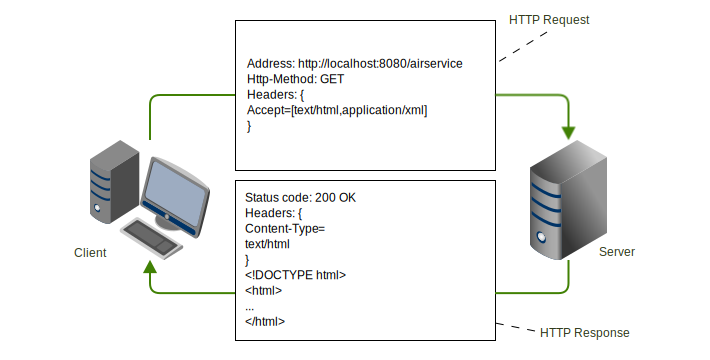
\includegraphics[width=13cm]{images-pdf/http.pdf}
\caption{Ukázka komunikace přes HTTP}
\label{fig:http-komunikace}
\end{center}
\end{figure}

HTTP je aktuálně velmi bohatý aplikační protokol poskytující množství zajímavých a
užitečných schopností. Na \ref{fig:http-komunikace} je zobrazen princip
komunikace přes HTTP. Podmínkou pro psaní RESTful aplikací je velmi dobrá
znalost HTTP protokolu.
HTTP je protokol s~určitými vlastnostmi (synchronní, požadavek/odpověď, aplikační, síťový) používaný pro distribuované spolupracující systémy. Jedná se o~primární
protokol používaný na webu, který je velmi jednoduchý - klient posílá požadavek složený
z~názvu HTTP metody, lokaci zdroje, hlavičky a volitelně z~těla požadavku, které může
obsahovat cokoliv. Nejčastěji se však pro tělo požadavku používá reprezentace dat v~JSON,
XML, HTML nebo prostém textu „plain text“.

\section{Rešerše generování vzdáleného API na platformě Java EE}

\subsection{Specifikace JAX-WS 2.0} 
\label{subsec:specifikace-jax-ws}

Specifikace JAX-WS \cite{JAXWS20} je standardizovaná technologie pro tvorbu SOAP-based
webových služeb na platformě Java. JAX-WS API skrývá aplikačnímu vývojáři svou
komplexitu.
Na serverové straně je třeba definovat interface\footnote{Publikovaná kompenenta
v~aplikaci definující zacházení s~aplikací} a v~něm metody, které se budou
mapovat na operace v~endpointu.

Specifikace nenutí, aby byly SOAP zprávy generovány a parsovány programově, protože
JAX-WS runtime systém převádí zprávy na Java objekty a obráceně za programátora.
V~některých situacích se však může stát, že je nutné zprávu generovat či parsovat ručně, což ale
JAX-WS umí, a to na různých úrovních abstrakce.

\subsubsection{Implementace endpointu webové služby}
\label{subsec:implementace-endpointu-webove-sluzby}

Výchozím bodem pro tvorbu JAX-WS webové služby je třída mající anotaci {\em
@WebService}, která je definována jako endpoint webové služby. SEI je Java
rozhraní či třída deklarující metody, které může klient konzumovat na
webové službě. Při tvorbě endpointu není povinné mít rozhraní, protože třída
implicitně definuje SEI. Pokud přeci jenom chceme oddělit funkcionalitu od
rozhraní, je nutné, kromě toho, aby třída implementovala {\em interface}, nastavit v~anotaci
{\em @WebService} v~elementu {\em endpointInterface} celý název rozhraní, tedy
i s~balíčkem.
Název služby (angl. {\em service name}) lze získat z~elementu {\em serviceName}
anotace {\em @WebService} a pokud je hodnota elementu prázdná, použije se název
implementující třídy s~příponou „Service“.

Pokud třída implicitně definuje SEI, jako webové operace budou namapovány metody
s~modifikátorem {\em public}, které splňují následující:
\begin{itemize}
  \item Metoda je anotována s~{\em @WebMethod}, jejíž element {\em exclude} je
  roven hodnotě {\em false}.
Defaultní hodnota je {\em false}, tudíž není povinné
element specifikovat.
  \item Metoda není anotována s~{\em @WebMethod} anotací, ale její deklarující třída má anotaci
{\em @WebService}.
\end{itemize}

Pro mapovací účely u~implicitního SEI jsou mapovány stejné anotace jako u~implementace
webové služby a jejích metod. Pokud nastane situace, že u~třídy anotované s~{\em @WebService}
chceme metodu s~modifikátorem {\em public} vynechat z~mapování na
operaci webové služby a máme SEI definované implicitně, musíme přidat k~metodě
anotaci {\em @WebMethod} a element {\em exclude} nastavit na {\em true}.
Pro mapovací účely musí být třída nejvyšší úrovně (angl. {\em top-level class})
nebo statická vnitřní třída.
Třída anotovaná {\em @WebService} musí mít defaultní veřejný konstruktor.

\subsubsection{Rozhraní endpointu webové služby}
SEI je mapováno na {\em wsdl:portType} element a jedná se o~Java
rozhraní, které splňuje následující omezení:

\begin{itemize}
  \item Musí být anotován s~{\em @WebService}.
  \item V~{\em @WebService} smí být vyplněn pouze element {\em targetNamespace}.
  \item Jakákoliv metoda může být anotována s~{\em @WebMethod}.
  \item Pokud je u~metody použita anotace {\em @WebMethod}, nesmí obsahovat
  element {\em exclude} s~hodnotou {\em true}.
  \item Všechny parametry a návratové typy musí být kompatibilní s~JAXB 2.0
  specifikací \cite{JAXB20}.
\end{itemize}

WSDL 1.1 nedefinuje standardní formu dědičnosti pro {\em wsdl:portType}
elementy.
Jediná povolená dědičnost je dědění Java metod s~JAX-WS anotacemi. I~když jsou metody
definovány v~jiném rozhraní než v~SEI, je s~nimi zacházeno, jako kdyby byly
definovány uvnitř SEI.

\subsubsection{Metoda}

Každá veřejná metoda v~SEI nemající anotaci {\em @WebMethod} s~elementem {\em
exclude} nastaven na {\em true}, je mapována na {\em wsdl:operation} element
v~korespondujícím {\em wsdl:portType}.

Jméno operace webové služby je mapováno z~elementu {\em name} v~anotaci {\em
@WebMethod} a pokud je element nespecifikován, použije se jméno Java metody.
Element {\em name} se používá k~řešení jmenných konfliktů, pokud existuje více
potencionálních operací webové služby se stejným
názvem.

Webové služby definují dva druhy metod - jednosměrné (angl. {\em
one-way}) a obousměrné (angl. {\em two-way}).
Jednosměrné mají vstup, ale neprodukují žádný výstup. Obousměrné mají vstup a
produkují výstup. Defaultně jsou všechny metody mapovány na obousměrné operace.
Pro definování jednosměrné operace stačí metodu anotovat s~{\em @OneWay}, ve
WSDL mají definován element {\em wsdl:input} definující vstupní parametry. Pro
obousměrné operace je navíc definován element {\em wsdl:output} za předpokladu, že Java metoda nevrací typ {\em void}.
Jsou u~nich definovány {\em wsdl:fault} elementy v~rozsahu nula až
vícekrát.
Element {\em wsdl:fault} je mapován z~výjimek definovaných v~metodě.

Jednosměrná metoda musí splňovat určitá kritéria. Pouze metody
s~návratovým typem {\em void}, které nemají parametr implementující {\em
Holder}, a které nevyhazují kontrolované výjimky, mohou, nikoliv musí, být jednosměrné.

Elementy {\em wsdl:input}, {\em wsdl:output} a {\em wsdl:fault} jsou asociovány
s~elementy {\em wsdl:message}, které definují přenášené zprávy. Hodnota atributu
{\em name} elementu {\em wsdl:message} není nijak důležitá a proto se používá
hodnota jména operace pro příchozí zprávy a hodnota jména operace zřetězená
s~„Response“ pro odchozí zprávy. U~zpráv typu {\em fault} se použije pro hodnotu
atributu název Java výjimky, pokud není specifikováno jinak v~anotaci {\em
@WebFault} u~metody.

Pro každý element {\em wsdl:message} lze definovat {\em Document} styl nebo RPC
styl.
V~Javě lze styl zpráv nakonfigurovat jak pro celý SEI, tak jednotlivě pro každou
metodu. Slouží k~tomu anotace {\em @SOAPBinding} a element {\em style}.

\subsubsection{Parametry a návratové typy}

Parametry a návratový typ Java metody jsou mapovány buď na zprávy, nebo na
deklarace globálních elementů. Pro přizpůsobení mapování parametru na zprávu je určena
anotace {\em @WebParam} a pro stejný účel slouží anotace {\em @WebResult}
u~návratového typu. Parametry mohou být mapovány na komponenty pro příchozí zprávy, odchozí zprávy nebo pro oboje.
Mapování záleží na klasifikaci parametru, který může být namapován jako SOAP
hlavička ve zprávě nastavením elementu {\em header} na {\em true} v~anotaci
{\em @WebParam}.
Element {\em header} v~anotaci {\em @WebResult} může být použit pro vložení
výsledku do SOAP hlavičky.

Parametry a návratové typy jsou rozděleny na tři módy podle toho, ve kterých zprávách se
vyskytují.

\begin{itemize}
  \item \textbf{\textit{In}} – hodnota je přenášena ve zprávě z~klienta na
  SEI, ale není přenášena zpět.
  \item \textbf{\textit{Out}} – hodnota je přenášena ve zprávě ze SEI ke
  klientovi, ale není přenášena zpět.
  \item \textbf{\textit{In/Out}} – hodnota je přenášena z~klienta na SEI a
  zpět ke klientovi.
\end{itemize}

Návratový typ je vždy mód {\em out}. U~parametrů, jejichž typ je obalen
třídou {\em Holder<T>}, je možno nastavit mód {\em in/out} nebo {\em out}.
U~ostatních parametrů je vždy použit mód {\em in}. Při obalení parametrů do Holder
můžeme docílit funkcionality, kterou Java neumí, a to vracet více hodnot
z~jedné metody. V~anotaci {\em @WebParam} se elementem {\em mode} nastavuje mód.

\subsubsection{Serializace dat}
\label{subsec:serializace-dat}

Pro definici serializace Java typů do SOAP zprávy je použita anotace {\em @SOAPBinding}, kterou
je možno použít u~třídy nebo metody.
Při užití na obou místech je upřednostněna ta u~metody. Anotace {\em @SOAPBinding} má
tři elementy s~možnými výčty hodnot popsanými
v~\ref{tab:soap-binding-vycet-hodnot}.

\begin{table}[h]
\begin{center}
\begin{tabular}{|c|l|l|}
\hline
\textbf{Element} & \textbf{Výčet hodnot} \\
\hline
Style & DOCUMENT, RPC \\
\hline
Use & LITERAL, ENCODING \\
\hline
ParameterStyle & WRAPPER, BARE \\
\hline
\end{tabular}
\end{center}
\caption{Výčet možných hodnot pro SOAP binding}
\label{tab:soap-binding-vycet-hodnot}
\end{table}

Kombinováním těchto tří elementů lze vytvářet odlišné struktury zpráv se stejnými nosnými
daty. Struktura zprávy je určena na základě zvolených hodnot v~elementech {\em @SOAPBinding}.

\subparagraph{Style}
% \begin{enumerate}
%   \item \textbf{\textit{Style}}
  	\begin{enumerate}[(a)]
  	  \item \textit{DOCUMENT} - obsah SOAP body bude XML dokument, který
  	  bude možno validovat vůči předdefinovanému XML Schema dokumentu.
  	  \item \textit{RPC} - SOAP body bude obsahovat XML reprezentaci volání
  	  metody.
Jako hlavní element se použije jméno metody a jako potomci parametry metody a
návratová hodnota.
	\end{enumerate}
\subparagraph{Use}
	\begin{enumerate}[(a)]
	  \item \textit{ENCODING} – udává, jak jsou hodnoty zakódovány do XML
	  formátu.
SOAP ENCODING je rozšíření SOAP Frameworku a nabízí pravidla, jak
konvertovat jakákoliv data ze SOAP datového modelu do XML formátu.
	  \item \textit{LITERAL} - definuje, že data jsou serializována podle
	  XML Schema.
	\end{enumerate}
\subparagraph{ParameterStyle}
	\begin{enumerate}[(a)]
	  \item \textit{WRAPPED} - říká, že zpráva bude zabalena ještě do
	  jednoho elementu.
	  \item \textit{BARE} - udává neobalování hodnot do jednoho hlavního
	  předka.
	\end{enumerate}

Přístup {\em DOCUMENT}/{\em LITERAL} je jednodušší přístup, protože se jednoduše
spoléháme na validaci zprávy vůči XML Schema.

Tvorba XML Schema z~Java typů je definována pomocí JAXB. Pomocí tohoto mapování
JAX-WS generuje do WSDL datové typy, které jsou užívány v~elementech {\em
message}. Jsou podporovány tři styly mapování: {\em document wrapped}, {\em
document bare} a RPC. Styly se liší v~XML Schema konstrukcích.

\textbf{\textit{Document wrapped}}

{\em Document wrapped} je definován v~anotaci {\em @SOAPBinding} s~následujícími
vlastnostmi:

\begin{itemize}
  \item \textbf{\textit{style}} – DOCUMENT,
  \item \textbf{\textit{use}} – LITERAL,
  \item \textbf{\textit{parameterStyle}} – WRAPPED.
\end{itemize}

Pro parametry se vytvoří wrapper\footnote{Obálka, do které jsou vloženy elementy
jako vnitřní prvky}, do kterého budou vygenerované typy umístěny a pro návratový
typ se vytvoří druhý wrapper. Jejich vlastnosti lze upravit v~anotacích
{\em @RequestWrapper} a {\em @ResponseWrapper}. Zde přicházejí do popředí módy
({\em in}, {\em out}, {\em in/out}):

\begin{itemize}
  \item Parametr s~módem {\em in} je mapován jako potomek globálního elementu
  request beany\footnote{Objekt vytvořený pomocí JAXB ze vstupu metody}.
  \item Parametr s~definovaným {\em out} nebo návratová hodnota jsou mapovány
  jako potomci response beany\footnote{Objekt vytvořený pomocí JAXB z~výstupu metody}.
  \item Parametr s~módem {\em in/out} je mapován jako potomek request beany i
  response beany.
\end{itemize}

\textbf{\textit{Document bare}}

Styl {\em document bare} je definován v~anotaci {\em @SOAPBinding}
s~následujícími vlastnostmi:

\begin{itemize}
  \item \textbf{\textit{style}} – DOCUMENT,
  \item \textbf{\textit{use}} – LITERAL,
  \item \textbf{\textit{parameterStyle}} – BARE.
\end{itemize}

Při aplikaci {\em document bare} jsou na metodu kladeny tyto požadavky:

\begin{itemize}
  \item Metoda musí mít maximálně jeden parametr {\em in} nebo {\em in/out},
  který není mapován na hlavičku.
  \item Pokud má návratový typ jiný než {\em void}, nesmí mít {\em in/out} a
  {\em out} parametry, které nejsou mapovány na hlavičky.
  \item Pokud má návratový typ {\em void}, může mít maximálně jeden parametr
  {\em in/out} nebo {\em out}, který není mapován na hlavičku.
\end{itemize}

Globální deklarace elementu je vygenerována pro vstupní typ metody a analogicky pro
výstupní typ metody.

\textbf{\textit{Styl RPC}}

Styl RPC je definován v~anotaci {\em @SOAPBinding} s~následujícími vlastnostmi:

\begin{itemize}
  \item \textbf{\textit{style}} – RPC,
  \item \textbf{\textit{use}} – LITERAL,
  \item \textbf{\textit{parameterStyle}} – WRAPPED.
\end{itemize}

Java typy pro parametry {\em in}, {\em in/out}, {\em out} a návratové
typy jsou mapovány na XML Schema typy s~použitím JAXB. Pro každý parametr metody a návratový typ je vytvořen ve WSDL
dokumentu element {\em part}, který je použit v~elementu {\em message}. Při
použití RPC stylu nesmí být posílány {\em null} hodnoty.

\subsection{Specifikace JAX-RS 2.0}
\label{subsec:specifikace-jax-rs}

Specifikace JAX-RS \cite{JAXRS20} byla vytvořena za účelem zjednodušení vývoje
RESTful služeb.
Použitím JAX-RS je webový zdroj (angl. {\em resource})  implementován jako
resource třída\footnote{Java třída využívající JAX-RS anotace pomocí,
kterých implementuje korespondující webový zdroj} a požadavky jsou obsluhovány resource
metodami\footnote{Java metoda resource třídy anotovaná JAX-RS
anotacemi, která obsluhuje HTTP požadavky}.

\subsubsection{Resource třída}
\label{subsec:resource-trida}

Resource třída je Java třída používající JAX-RS anotace k~implementaci
konkrétního webového zdroje. Musí splňovat požadavek na POJO třídu a zároveň
musí mít alespoň jednu metodu s~anotací {\em @Path} nebo s~anotací obsahující
request method designator\footnote{Runtime anotace anotovaná s~{\em
@HttpMethod}.
Používá se pro identifikaci jaký typ HTTP metody může resource metoda
obsloužit.}.
Pokud není explicitně změněno, nová instance resource třídy je vytvořena
pokaždé, když přijde požadavek na webový zdroj, jenž třída implementuje.
Implementace JAX-RS může kromě životního cyklu {\em per-request} poskytovat
jeho další volby. Speciální resource třídou je kořenová resource
třída\footnote{Je to resource třída anotovaná {\em @Path}. Kořenová resource
třída je výchozím bodem pro adresy subzdrojů.}.
Aby se resource třída mohla stát kořenovou, musí obsahovat anotaci {\em @Path}
s~URI, na které bude tato root resource třída zaregistrována a kde bude vyřizovat požadavky. \cite{JAXRS20}

\subsubsection{Konstruktor}

Root resource třída je instanciovaná JAX-RS runtimem a musí mít konstruktor
s~modifikátorem {\em public}, který může být bezparametrický nebo parametrický.
Může obsahovat takové parametry, aby je JAX-RS runtime byl schopen předat konstruktoru. Jako parametry
může konstruktor obsahovat ty, které jsou anotovány {\em @Context}, {\em @HeaderParam},
{\em @CookieParam}, {\em @MatrixParam}, {\em @QueryParam} a {\em @PathParam}. Pokud je obsaženo více
veřejných konstruktorů, použije se ten, který obsahuje nejvíce parametrů. Při
shodě počtu parametrů dvou konstruktorů není pořadí jednoznačně určeno a implementace JAX-RS si
mohou zvolit, který z~nich použijí, zároveň by však měly generovat varování
o~této víceznačnosti. Resource třída, která není kořenová, je instanciovaná
aplikačním kódem a nepotřebuje výše popisovaný veřejný konstruktor.

\subsubsection{Atributy}
\label{ch:atributy}

Při vytváření instance resource třídy lze naplnit její atributy konstruktorem nebo setter
metodami. Pokud má atribut modifikátor {\em public}, lze přidat anotace přímo
k~atributu. Anotace jsou stejné u~všech tří zmíněných přístupů plnění hodnot - {\em @Context}, {\em @HeaderParam},
{\em @CookieParam}, {\em @MatrixParam}, {\em @QueryParam} a {\em @PathParam}. Protože injektování probíhá
při tvorbě objektu, je použití těchto anotací (s~výjimkou {\em @Context})
v~resource třídě u~konstruktoru a při nastavování atributů podporováno pouze u~{\em per-request}
životního cyklu. Objekty vrácené pomocí sub-resource lokátoru\footnote{Metoda
resource třídy používaná k~lokaci subzdrojů korespondujícího zdroje.} se
inicializují programově přímo v~kódu, nejsou tedy ve správě JAX-RS runtime.

Typy, pro které mohou být použity anotace {\em @HeaderParam}, {\em @CookieParam}, {\em @MatrixParam},
{\em @QueryParam} a {\em @PathParam}, musí splňovat jednu z~následujících podmínek:

\begin{enumerate}
  \item Typy, pro které je {\em ParamConverter} definován pomocí registrace
  {\em ParamConverterProvider}.
  \item Primitivní typy.
  \item Typy mající konstruktor, který obsahuje jeden parametr typu {\em
  String}.
  \item Typy mající statickou metodu pojmenovanou {\em valueOf} nebo {\em
  fromString} s~jedním parametrem typu {\em String} a návratovou hodnotou
  vracející instanci daného typu. Pokud typ není {\em enum}, musí být při
  výskytu obou metod současně upřednostněna {\em valeuOf}. V~případě {\em enum}
  má přednost {\em fromString} metoda.
  \item {\em List<T>}, {\em Set<T>} nebo {\em SortedSet<T>}, kde T vyhovuje bodu
  3 nebo 4.
\end{enumerate}

Anotace {\em @DefaultValue} může být použita pro případ, kdy atribut nedostane
žádnou hodnotu.
Anotace přijímá hodnotu jako {\em String} a ten je poté převáděn do požadované
podoby pomocí kroků 1 - 5 výše.

\subsubsection{Resource metoda}
\label{subsec:resource-metoda}

Resource metoda je metoda obsluhující požadavek, který přišel na resource třídu. Tato metoda
musí mít anotaci request method designatoru. Taková anotace má anotaci {\em
@HttpMethod} a JAX-RS definuje množinu request method designátorů pro obecně
definované HTTP metody.
Jejich anotace jsou následující {\em @GET}, {\em @POST}, {\em @PUT}, {\em
@DELETE}, {\em @HEAD}, {\em @OPTIONS}.
Lze si zadefinovat designator pro vlastní HTTP metodu tím, že se vytvoří anotace mající
anotaci {\em @HttpMethod}. Pouze metody, které mají modifikátor přístupu {\em
public}, mohou být považovány za resource metody.

Po invokaci resource metody jsou parametry anotované {\em @Context}, {\em @HeaderParam},
{\em @CookieParam}, {\em @MatrixParam}, {\em @QueryParam}, {\em @PathParam} a {\em @FormParam} mapovány
z~požadavku podle sémantiky anotace. Podobně jako u~atributů je zde možno použít anotaci
{\em @DefaultValue}. Parametr nemající výše uvedenou anotaci je označován jako
entity parametr\footnote{Parametr metody, který není anotován request method
designatorem. Je mapován z~těla požadavku.} a je mapován z~těla požadavku.
Za převody mezi tělem požadavku a Java typem jsou zodpovědní entity
provideři\ref{subsec:entity-provideri}.
Resource metoda může mít maximálně jeden entity parametr.

Resource metoda může vracet návratový typ {\em void}, {\em Response},
{\em GenericEntity} nebo jiný Java typ. Tyto typy jsou mapovány do těla odpovědi
následovně:

\begin{itemize}
  \item \textbf{\textit{Void}} – prázdné tělo odpovědi se status kódem 204.
  \item \textbf{\textit{Response}} – tělo odpovědi je naplněno z~entity
  property objektu typu {\em Response} se status kódem specifikovaným ve status property objektu typu {\em Response}. Pokud je
návratová hodnota {\em null}, status kód bude 204. Při {\em non-null} entity
property v~{\em Response} a nespecifikovaném statusu je status nastaven na 200.
Při {\em null} entity property je status nastaven na 204.
  \item \textbf{\textit{GenericEntity}} – tělo odpovědi je naplněno
  z~entity property objektu typu {\em GenericEntity}. Při {\em null} těle
  odpovědi je status 204, při {\em non-null} 200.
  \item \textbf{\textit{Ostatní}} – tělo odpovědi je přímo mapováno
z~instance, která se vrací.
Pokud je vrácena instance anonymní vnitřní třídy, je použit její předek. Při
{\em null} je status 204, jinak 200.
\end{itemize}

Metody, které potřebují posílat více metadat než jen tělo odpovědi a status kód, by měly
vracet instanci třídy {\em Response}.

\begin{table}
\begin{center}
\begin{tabular}{|c|l|l|l|}
\hline
\textbf{Návratový typ} & \textbf{Návratová instance} & \textbf{Raw typ} &
\textbf{Generický typ} \\
\hline
GenericEntity & GenericEntity nebo podtřída & RawType property & Type property \\
\hline
Response & GenericEntity nebo podtřída & RawType property & Type property \\
\hline
Response & Object nebo podtřída  & Třída instance & Třída instance \\
\hline
Jiný & Návratový typ nebo podtřída  & Třída instance & Generický typ \\
&&&  vráceného typu \\
\hline
\end{tabular}
\end{center}
\caption{Určení generických a raw typů návratových hodnot}
\label{tab:genericke-a-raw-typy}
\end{table}

Sub-resource metody a sub-resource lokátor metody mohou vyhazovat očekávané
nebo neočekávané výjimky. Tyto výjimky musí být runtimem namapovány na HTTP odpověd.

Očekávanou výjimku lze přebalit do instance {\em WebApplicationException} a
jejích podtříd nebo je možné implementovat pro výjimku exception
mapper\footnote{Java třída provádění mapování výjimky na HTTP odpověď.}, kterému
bude jako parametr předána výjimka a na základě ní bude vytvořena požadovaná
odpověď.

Root resource třída je ukotvena v~URI prostoru použitím anotace {\em @Path}.
Hodnota v~anotaci je relativní URI šablona cesty, jejíž základní URI je postavena z~deployment kontextu a cesty
aplikace. Šablona URI cesty je textový řetězec se žádným nebo více vloženými
parametry. Po dosazení konkrétních hodnot za parametry se ze šablony stane validní URI cesta. Parametr
v~šabloně cesty je umístěn ve složených závorkách \{\}. Parametr v~URI šabloně
může specifikovat i regulární výraz. Například {\em @Path(„test/{id:.+}“)} říká,
že resource třída či metoda bude vyhovovat, pokud URI bude začínat na test a poté bude následovat alespoň jeden
segment cesty. V~tomto případě lze parametr {\em id} nainjektovat jako atribut
třídy nebo parametr metody pomocí anotace {\em @PathParam}.

Metody v~resource třídě mající anotaci {\em @Path} mohou být buď sub-resource
metodami nebo sub-resource lokátory. Sub-resource metody odchytí a zpracují HTTP požadavek přímo uvnitř
metody, zatímco sub-resource lokátor metoda vytvoří a vrátí instanci, která obslouží HTTP
požadavek. Zda-li se jedná o~první nebo druhý typ, je řízeno přítomností request method
designatoru. Pokud je designator přítomný, jedná se o~sub-resource metodu a ta přímo
obslouží požadavek a vrátí například instanci {\em Response}. Při absenci designatoru se dynamicky
rozhodne o~objektu, na který bude delegováno obsloužení požadavku. Při vyřizování
požadavku je objekt považován za resource třídu a může mít stejné anotace jako resource
třída. Sub-resource lokátor metoda může mít stejné parametry jako normální resource metoda,
ale nesmí obsahovat entity body parametr.

U~resource metod a resource třid lze definovat formát akceptovatelný pro
požadavek i formát, jenž bude navrácen v~odpovědi. Pokud je nadefinován formát
u~třídy i metody, má přednost formát u~metody. Při nedefinovaném formátu
u~metody se akceptují ty, které jsou definovány u~třídy. Pokud není formát
definovaný ani ve třídě, použije se formát {\em „*/*“}. V~HTTP protokolu se pro
práci s~formáty používají dvě hlavičky, jsou jimi {\em Content-Type} a {\em
Accept}.
{\em Content-Type} obsahuje formát přenášeného obsahu s~touto hlavičkou a {\em
Accept} říká, jaký formát chce posílající přijmout. V~JAX-RS těmto hlavičkám
odpovídají anotace {\em @Consumes} a {\em @Produces}. {\em @Consumes} odpovídá
hlavičce {\em Accept} a {\em @Produces} hlavičce {\em Content-Type}.

\subsubsection{Dědičnost resource tříd}
\label{subsec:dedicnost-resource-trid}

JAX-RS anotace mohou být užity nejen přímo v~resource třídě, ale také
v~nadtřídách a rozhraních, jež implementují. Proto je nutné specifikovat pořadí,
v~jakém budou mít anotace přednost. Největší přednost mají anotace přímo
v~resource třídě. Pokud u~resource třídy nebo u~resource metody nějaké jsou, jsou
ostatní třídy a rozhraní ignorovány. Dalším pravidlem je, že má vždy přednost
nadtřída před rozhraním a nezáleží na tom, jak je třída vysoko. V~řetězu tříd
dědičnosti seřazeném od nejobecnější po nejkonkrétnější třídu má vždy
větší prioritu ta, která je konkrétnější. Jelikož jedna třída může mít maximálně
jednoho přímého předka, nemůže zde nastat kolize. Pokud by každá třída
implementovala pouze jeden interface, kolize by také nemohla nastat a přednost
by měly anotace z~interfacu, který je nejblíže třídě. Pokud je na jedné úrovni
více rozhraní, není jejich přednost specifikována a každý
implementátor JAX-RS si může zvolit vlastní pořadí.

\subsubsection{Entity provideři}
\label{subsec:entity-provideri}

V~JAX-RS existují entity provideři, kteří se starají o~mapování přenášených
dat na Java objekty a obráceně. Jedním typem entity providerů je {\em
MessageBodyReader} a druhým je {\em MessageBodyWriter}.  Rozhraní 
{\em MessageBodyReader} definuje kontrakt mezi JAX-RS runtime a komponentami
mapující data na Java objekty, rozhraní {\em MessageBodyWriter} definuje
obrácený směr mapování.

\paragraph{MessageBodyReader}
\label{par:messagebodyreader}
\mbox{}\\

Java třídy poskytující tuto funkcionalitu musí implementovat rozhraní
{\em MessageBodyReader} a mohou být anotovány s~{\em @Provider} pro automatické
zaregistrování.

Následující body popisují kroky provedené JAX-RS implementací při mapování
entity body na parametr Java metody:

\begin{enumerate}
  \item Získání media typu požadavku. Pokud požadavek neobsahuje HTTP hlavičku
{\em Content-Type}, pak je použit {\em application/octet-stream}.
  \item Identifikace Java typu parametru metody.
  \item Provedení výběru množiny možných {\em MessageBodyReader} providerů,
  kteří podporují media typ požadavku.
  \item Iterování přes vybrané {\em MessageBodyReader} třídy a zavolání metody
  {\em isReadable}.
Provede se výběr nejvhodnějšího {\em MessageBodyReader} providera, který
podporuje již zmíněný Java typ.
  \item Pokud předchozí krok vybral vhodného {\em MessageBodyReader} providera,
  pak je použita jeho metoda {\em readFrom} pro namapování entity body na
  požadovaný Java typ.
  \item V~opačném případě musí server runtime vygenerovat výjimku {\em
  NotSupportedException} se statusem 415.
\end{enumerate}

\paragraph{MessageBodyWriter}
\mbox{}\\

Zaregistrování {\em MessageBodyWriter} providera je stejné jako pro
{\em MessageBodyReader} (viz kapitola \ref{par:messagebodyreader}).

Následující body popisují kroky provedené JAX-RS implementací při mapování
návratového hodnoty na entity body:

\begin{enumerate}
  \item Získání objektu, který bude mapován na entity body. Pro návratový typ {\em Response} a
jeho podtříd je objekt získán z~property entity.
  \item Dojde k~určení media typu pro odpověď.
  \item Vybere se množina {\em MessageBodyWriter} providerů, kteří podporují typ
  vráceného objektu a media typ.
  \item Seřadí se vybraní {\em MessageBodyWriter} provideři primárně podle
  podporovaného generického typu od toho, který je nejblíže vrácenému objektu, a
  sekundárně podle podporovaného media typu.
  \item Iterace přes všechny seřazené {\em MessageBodyWriter} providery a
  zavolání metody {\em isWritable}. Následně dojde k~vybrání nejvhodnějšího
  {\em MessageBodyWriter}.
  \item Pokud v~předchozím kroku došlo k~vybrání vhodného kandidáta, použije se
metoda {\em writeTo} k~namapování objektu na entity body.
  \item V~opačném případě musí server runtime vygenerovat {\em
  InternalServerErrorException}, což je podtřída {\em WebApplicationException}
  se statusem 500.
\end{enumerate}

\subsection{Apache Maven}

Velká většina Maven \cite{Maven08} uživatelů označuje Maven za sestrojovací nástroj,
což není zcela správně, protože Maven umí více než jen tvorbu artefaktů ze zdrojových kódů. Typickým představitelem
kategorie sestavovacích nástrojů je Apache Ant \cite{AntHome}. Při srovnání těchto dvou
nástrojů je patrné, jaké funkcionality má Maven oproti klasickému sestavovacímu
nástroji navíc. Klasický sestavovací nástroj provádí preprocessing, kompilaci, zabalení, testování a distribuci. Maven může navíc tvořit reporty,
generovat webové stránky a usnadňuje komunikaci mezi ostatními členy týmu. Správné
označení pro Maven je tedy project management tool.

\subsubsection{Konvence a jednotné rozhraní}

Nástroj Maven jako první zavedl konvence a jednotné rozhraní. Díky němu se
vyvarujeme tomu, aby člověk, který je u~projektu nový, strávil hodiny studováním
sestavení.
Maven defaultně definuje, ve kterých adresářích má být uložen zdrojový kód ({\em
\${basedir}/src/main/java}), ostatní zdroje ({\em
\${basedir}/src/main/resources}) nebo zdrojové kódy pro testy ({\em
\${basedir}/src/test}). Dále jsou také definovány defaultní umístění pro
zkompilované třídy ({\em \${basedir}/target/classes}) a zabalený artefakt ({\em
\${basedir}/target}). S~použitím Mavenu se již nemusí ručně stahovat všechny
závislosti pro knihovnu, kterou jsme se rozhodli použít, jelikož jsou tyto
závislosti automaticky získány z~repozitáře. Maven definuje také životní cyklus
sestavení, který se skládá z~po sobě jdoucích fází.
Pokud se člověk dostane k~projektu používající Maven, nejenže se hned orientuje
v~adresářové struktuře, ale pro spuštění celého sestavení stačí zadat příkaz
{\em mvn install}.

\begin{code}[frame=single, caption={Defaultní adresářová struktura Maven
projektu}, label={lst:maven-dirs}] pom.xml
src/
  main/
    java/
    resources/
  test/
    java/
    resources/
target/
  classes/
  deployable artifact (JAR, EAR, WAR, ...)
\end{code}

Zde je popsána struktura z~\ref{lst:maven-dirs}. Soubor {\em pom.xml} je Maven
konfigurační soubor daného projektu.
Adresář {\em java} obsahuje zdrojové kódy, adresář {\em resources} pak ostatní zdroje mimo
zdrojové kódy (konfigurační soubory, descriptoty, obrázky atd...). Adresář {\em
classes} obsahuje zkompilovaný kód. Deployable artifact může být výsledný soubor
jar, war či ear.

\subsubsection{Project Object Model (POM)}

Apache Maven udržuje model projektu, nestará se pouze o~kompilování kódu do bajtkódu.
Udržuje název projektu, licenci pod kterou je software vyvíjen, kdo stojí za vývojem projektu,
kdo přispívá do projektu a na kterých projektech je tento projekt závislý. Maven drží
informaci, jakým SCM je projekt verzován a na jaké adrese lze nalézt repozitář. Všechny tyto
informace jsou konfigurovány v~souboru pom.xml, který je povinný pro každý projekt. Každý
projekt v~Mavenu je jednoznačně identifikovatelný, protože má Maven coordinates, které se
skládají z~{\em groupId}, {\em artifactId} a {\em version}. 
{\em GroupId} uvozuje skupinu, pod kterou projekt patří (například
{\em org.apache.maven}), {\em artifactId} blíže identifikuje projekt v~rámci
{\em groupId} (například {\em maven-plugin-api}) a {\em version} udává verzi projektu
(například {\em 1.0.0}).

\subsubsection{Maven repozitář}

Při prvním spuštění Mavenu začne Maven stahovat závislosti z~místa nazývaného Maven
repozitář. Repozitář je zdroj v~síti, kde jsou uchovávány artefakty (jar, war,
ear, maven pluginy atd...), které jsou uloženy v~adresářové struktuře podle Maven coordinates. Centrální
repozitář se nachází na {\em http://repo1.maven.org/maven2}. Knihovny, které
potřebuje projekt, se nacházejí právě v~takových repozitářích. Potřebnou knihovnu není třeba
stahovat ručně, ale pouze se v~pom.xml do elementu {\em dependencies} přidají
coordinates požadované knihovny, která se při spuštění sestavení automaticky získá.

Aby se při každém sestavení nemuseli všechny závislosti opakovaně stahovat, na
lokální stanici se vytváří lokální repozitář na cestě {\em
/home/USERNAME/.m2/repository}, kde se ukládají artefakty. Maven vždy hledá
artefakt v~lokálním repozitáři a až poté prohledává ty vzdálené. Při spuštění
{\em mvn install} se v~poslední fázi sestavení nainstaluje nově vytvořený
artefakt do lokálního repozitáře pro použití v~dalších projektech. Pokud projekt obsahuje
závislost mající další závislosti, jsou automaticky získány všechny. Strom
závislostí lze zobrazit spuštěním {\em mvn dependency:tree}, což lze
vysvětlit jako spuštění pluginu {\em dependency} s~goalem {\em tree}.

\subsubsection{Životní cyklus}

Životní cyklus sestavení je seřazená sekvence fází (angl. {\em phases}) zahrnutá
v~sestavování projektu. Maven může podporovat různé životní cykly, ale defaultní
životní cyklus začíná validací základní integrity projektu a končí fází deployování do produkčního prostředí.

Seznam fází defautního životního cyklu:

\begin{itemize}
  \item \textbf{\textit{validate}} – ověření, že projekt nemá žádné
  chyby a všechny potřebné informace jsou v~něm dostupné,
  \item \textbf{\textit{compile}} – kompilování zdrojových kódů,
  \item \textbf{\textit{test}} – testování zkompilovaného kódu s~použitím
  testovacího frameworku. Tyto testy nevyžadují, aby byl kód zabalen nebo deployován,
  \item \textbf{\textit{package}} – vezme zkompilovaný kód a zabalí ho do
  distribuovatelného formátu, například jako jar,
\item \textbf{\textit{integration-test}} – distribuce balíčku na
prostředí, kde mohou proběhnout integrační testy, provedení testů,
\item \textbf{\textit{verify}} – kontroly k~ověření validnosti balíčku a
splnění kvality,
\item \textbf{\textit{install}} – instalace balíčku do lokálního repozitáře
k~použití v~jiných projektech,
\item \textbf{\textit{deploy}} – v~integračním nebo release prostředí
zkopíruje balíček do vzdáleného repozitáře pro sdílení s~ostatními projekty a
vývojáři.
\end{itemize}

Seznam fází není kompletní a může se rozrůst. Pokud chceme projekt dostat do určité fáze
(nemusí se nutně jednat o~poslední fázi), stačí zadat jméno poslední fáze, která se má spustit a
Maven automaticky začne spouštět fáze od první až po explicitně vyvolanou. Co se děje
v~jednotlivých fázích, je popsáno v~kapitole \ref{subsec:pluginy-a-goaly}.

\subsubsection{Pluginy a goaly}
\label{subsec:pluginy-a-goaly}

Goal je specifická úloha obsažená v~Maven pluginu, kterou je možné spustit.
Vhodným příkladem může být jednoduchý {\em maven-jar-plugin}, který má {\em
pluginId} jar a goal jar. Plugin může být spuštěn příkazem {\em mvn
pluginId:goal} nebo může být připojen k~určité fázi životního cyklu.
Vyvoláním fáze se spustí plugin s~určitým goalem. Celý životní cyklus sestavení
je v~podstatě postupné spouštění různých goalů z~různých pluginů. Goaly je možno
konfigurovat v~pom.xml.

\begin{code}[frame=single,caption={Ukázka konfigurace v~pluginu}]
<plugin>
  <groupId>org.apache.maven.plugins</groupId>
  <artifactId>maven-compiler-plugin</artifactId>
  <version>3.1</version>
  <configuration>
    <source>1.6</source>
    <target>1.6</target>
    <debug>true</debug>
  </configuration>
</plugin>
\end{code}

Konfiguraci goalu lze umístit na různá místa v~konfiguračních pom.xml souborech,
čímž je myšleno, do kterého XML elementu se má umístit element {\em
configuration}.
Element {\em configuration} uvnitř sebe obsahuje další elementy, které
reprezentují danou konfiguraci. Při globální konfiguraci pluginu je konfigurace
umístěna do elementu {\em plugin}. Tato konfigurace bude společná pro všechny
goaly uvnitř pluginu. Další možností je umístit konfiguraci pouze ke konkrétnímu
goalu, což se provede vložením konfigurace do elementu {\em execution}, který
obsahuje informaci, ke kterému goalu se vztahuje. Pokud plugin obsahuje konfiguraci na
obou místech, ke konfiguraci goalu, která má přednost, se aplikuje konfigurace
pluginu.
Aplikovány budou pouze ty konfigurační elementy pluginu, které nepřepisují
konfigurační elementy goalu. Situace se trochu zkomplikuje při multimodulových
projektech, kde je plugin nakonfigurován v~rodičovském modulu i v~potomkovi.
Jelikož Maven tvoří efektivní pom, přidá konfiguraci pluginu, resp. goalu
z~rodiče do konfigurace pluginu, resp. goalu potomka.
Seřazená konfigurace od nejobecnější k~nejkonkrétnější vypadá takto: konfigurace
pluginu v~rodiči, konfigurace pluginu v~potomkovi, konfigurace goalu v~rodiči a
konfigurace goalu v~potomkovi.

\subsubsection{Multimodulový projekt}

Multimodulový projekt je definován rodičovským pomem, uvnitř kterého jsou definovány
jeho submoduly. Rodičovský pom bývá též nazývaný top-level pom.

\begin{code}[frame=single,caption={Ukázka konfigurace multimodulového
projektu}] 
<?xml version="1.0" encoding="UTF-8"?>
<project xmlns="http://maven.apache.org/POM/4.0.0"
         xmlns:xsi="http://www.w3.org/2001/XMLSchema-instance"
         xsi:schemaLocation="http://maven.apache.org/POM/4.0.0
         http://maven.apache.org/xsd/maven-4.0.0.xsd">
    <modelVersion>4.0.0</modelVersion>

    <groupId>org.jrapidoc</groupId>
    <artifactId>jrapidoc-pom</artifactId>
    <version>1.0-SNAPSHOT</version>

    <packaging>pom</packaging>

    <modules>
        <module>jrapidoc-rest-plugin</module>
        <module>jrapidoc-soap-plugin</module>
        <module>jrapidoc-annotation</module>
        <module>jrapidoc-gui</module>
        <module>jrapidoc-model</module>
        <module>jrapidoc-logger</module>
        <module>jrapidoc-plugin-base</module>
    </modules>

    <build>
        <pluginManagement>
            <plugins...>
        </pluginManagement>
    </build>

    <dependencyManagement>
        <dependencies...>
    </dependencyManagement>
</project>
\end{code}

Rodič definuje Maven coordinates ({\em groupId}, {\em artifactId} a {\em
version}).
Top-level projekt nevytváří artefakty JAR, WAR a podobné, o~to se starají submoduly. Top-level projekt definuje
submoduly a provádí globální konfiguraci, která je společná submodulům. Například mohou
být definovány společné závislosti pomocí coordinates knihoven, poté pracují submoduly se
stejnou verzí knihovny. Pokud je provedeno sestavení v~top-level projektu,
všechny submoduly budou také sestaveny.

\subsubsection{Vlastní plugin}

Maven plugin se skládá z~plugin descriptoru a jednoho nebo více MOJO. Maven běží
uvnitř IoC kontejneru Plexus \cite{PlexusHome}, který se stará o~injektování komponent,
které jsou definovány v~MOJO třídě. MOJO třída je třída implementující rozhraní {\em Mojo},
který obsahuje výchozí metodu {\em execute}, jež je výchozím bodem pro každý
plugin.
Komponenty mohou být v~MOJO třídě buď Java primitivní typy, soubory, pole, MOJO
třídy nebo reference na jiný projekt, než ve kterém je plugin spuštěn.

Plugin descriptor, který je povinný v~každém modulu, obsahuje konfiguraci pluginu. Je
umístěn v~{\em META-INF/maven/plugin.xml} Tento descriptor není nutné psát
ručně, ale lze jej generovat pluginem {\em maven-plugin-plugin} a jeho goalem
{\em descriptor}. Descriptor je generován na základě introspekce kódu.

\begin{code}[frame=single,caption={Ukázka plugin descriptoru}]
<?xml version="1.0" encoding="UTF-8"?>
<plugin>
  <name>jrapidoc-rest-plugin</name>
  <description></description>
  <groupId>org.jrapidoc</groupId>
  <artifactId>jrapidoc-rest-plugin</artifactId>
  <version>1.0-SNAPSHOT</version>
  <goalPrefix>jrapidoc-rest</goalPrefix>
  <isolatedRealm>false</isolatedRealm>
  <inheritedByDefault>true</inheritedByDefault>
  <mojos>
    <mojo>
      <goal>run</goal>
      <description>Created by papa on 14.3.15.</description>
      <requiresDirectInvocation>false</requiresDirectInvocation>
      <requiresProject>true</requiresProject>
      <requiresReports>false</requiresReports>
      <aggregator>false</aggregator>
      <requiresOnline>false</requiresOnline>
      <inheritedByDefault>true</inheritedByDefault>
      <phase>process-classes</phase>
      <implementation>org.jrapidoc.plugin.RestMojo</implementation>
      <language>java</language>
      <instantiationStrategy>per-lookup</instantiationStrategy>
      <executionStrategy>once-per-session</executionStrategy>
      <threadSafe>false</threadSafe>
      <parameters>
        <parameter>
          <name>baseUrl</name>
          <type>java.lang.String</type>
          <required>false</required>
          <editable>true</editable>
          <description></description>
        </parameter>
        <parameter>
          <name>custom</name>
          <type>java.util.Map</type>
          <required>false</required>
          <editable>true</editable>
          <description></description>
        </parameter>
    ...dalsi parametry
      </parameters>
      <configuration>
        <basedir implementation="java.io.File" 
        default-value="${project.basedir}"/>
        <target implementation="java.io.File" 
        default-value="${project.build.directory}"/>
      </configuration>
    </mojo>
  </mojos>
  <dependencies...>
</plugin>
\end{code}

Postup při tvorbě pluginu spočívá v~založení Maven projektu s~{\em packaging}
nastaveným na {\em maven-plugin}. Dalším krokem je nakonfigurování potřebných
pluginů a závislostí v~pom.xml.
Po splnění těchno prerekvizit je možné tvořit MOJO třídy.

\paragraph{Anotace v~MOJO}
\mbox{}\\

Ke třídě MOJO se váže nejdůležitější anotace {\em @Mojo}, některé její elementy
zde budou vysvětleny. Element {\em name} udává jméno goalu, který bude
reprezentován MOJO třídou.
Element {\em defaultPhase} specifikuje defaultní fázi, ke které bude goal
napojen, pokud nebude explicitně definováno v~konfiguraci jinak. Element
{\em requiresDependencyResolution} definuje, jaké závislosti bude plugin mít na
classpath při spuštění. Možné volby jsou: {\em NONE}, {\em COMPILE},
{\em COMPILE\_PLUS\_RUNTIME}, {\em RUNTIME}, {\em RUNTIME\_PLUS\_SYSTEM} a {\em
TEST}.

\paragraph{Parametry v~MOJO}
\mbox{}\\

Další důležitou částí vedle metody execute() a anotací jsou v~MOJO třídě parametry. Parametry
se do MOJO dostanou z~konfigurace pluginu v~pom.xml pomocí IoC kontejneru Plexus.

\begin{code}[frame=single,caption={Definice parametru
v~Mojo},label={lst:parametr-v-mojo}] 
@Parameter(defaultValue = "${project.basedir}", readonly = true) 
File basedir;
\end{code}

V~ukázce \ref{lst:parametr-v-mojo} je vidět, jak se definuje instanciování
objektu typu {\em File} reprezentujícího kořenový adresář projektu. Hodnota
elementu {\em defaultValue} obsahuje ve složených závorkách jméno maven
property, ve které je uložena cesta k~tomuto adresáři. Parametry mohou být i
vícehodnotové, což je užitečné v~případě, kdy je třeba do konfigurace přidat
parametr typu pole nebo {\em List} a podobné. Co je pro to nutné udělat, je
vidět na ukázkách \ref{lst:mojo-vicehodnotovy-parametr} a na
\ref{lst:pom-vicehodnotovy-parametr}.

\begin{code}[frame=single,caption={Definice vícehodnotového parametru
v~Mojo},label={lst:mojo-vicehodnotovy-parametr}] 
@Parameter(name = "includes")
List<String> includes;
\end{code}

\begin{code}[frame=single,caption={Konfigurace vícehodnotového parametru
v~pom.xml},label={lst:pom-vicehodnotovy-parametr}] 
<includes>
    <include>airservice.resources</include>
    <include>airservice.otherresources</include>
</includes>
\end{code}

V~definici parametru pro MOJO je podporován i typ {\em Map<String, String>}.
Konfigurace takového parametru vypadá podobně jako konfigurace pro pole, ale místo názvů elementů
include z~ukázky \ref{lst:pom-vicehodnotovy-parametr} se použijí klíče pro mapu.

\section{Rešerše existujících generátorů dokumentace}
\label{sec:reserse-existujicich-generatoru}

Cílem rešerše existujících nástrojů je prozkoumat ty nástroje, které umí
dokumentovat RESTful rozhraní, SOAP-based webové služby. Analyzovány budou
takové nástroje, které umí provádět generování ze specifikací JAX-WS a JAX-RS.
Jelikož popis některých částí rozhraní není možné staticky vyčíst z~analýzy
kódu, je nutné zjistit, jak jsou v~jednotlivých nástrojí tyto situace řešeny.

Na základě pozitiv a negativ, které budou u~jednotlivých nástrojů zjištěny, bude stanoveno,
jaké funkce bude mít nově vznikající nástroj.

\subsection{Swagger}
\label{subsec:swagger}

Swagger \cite{SwaggerHome} je nástroj pro tvorbu API dokumentace a testovacího
klienta a pracuje pouze s~RESTful službami.
V~současné době je zřejmě nejoblíbenějším nástrojem pro API dokumentaci. Do
zdrojového kódu přidává vlastní anotace, které pomáhají vytvořit kvalitnější API
dokumentaci. Swagger při generování artefaktů vytváří soubory podobným
principem, jako je vytvořeno WSDL u~SOAP-based webových služeb. Vygenerované
soubory jsou ve formátu JSON. Pro každou resource třídu je jeden soubor, na
který odkazuje hlavní soubor service.json, jež slouží jako výchozí bod se
seznamem zdrojů. Vygenerované artefakty tvoří model rozhraní\footnote{Datová
struktura reprezentující popis vzdáleného rozhraní}, který je načítán klientem,
jež umožňuje zobrazit API dokumentaci.
Klient je grafické rozhraní v~HTML, CSS a JavaScriptu. Pokud chceme provolat
metody, musíme vygenerovaný model načíst v~Swagger UI. Swagger UI je grafické
rozhraní podobné klientovi.

Swagger bude pro svou oblibu analyzován mnohem podrobněji než ostatní nástroje.

\paragraph{Výhody}
% \textbf{\textit{Výhody}}

\begin{itemize}
  \item Pod Apache License, Version 2.0 \cite{ApacheLic04}.
  \item Dokáže provolat metody z~API.
  \item Tvorba modelu rozhraní z~různých jazyků (Java, Scala, .NET, Go, JavaScript, PHP,
Python, \ldots).
  \item Tvorba klienta v~různých jazycích (Java, Scala, .NET, Go, JavaScript, PHP, Python,
\ldots).
\item Integrace s~Apache Maven.
\end{itemize}

\paragraph{Nevýhody}

\begin{itemize}
  \item Podpora pouze RESTful služeb.
  \item Složitá konfigurace.
  \item Nepodporuje dostatečně JAX-RS.
  \begin{itemize}
    \item Nepodporuje dědičnost u~resource tříd. Pokud dědičnost existuje, skončí chybou a
nezobrazí v~GUI u~zdroje žádné metody.
    \item Nepodporuje sub-resource lokátor. Pokud sub-resource lokátor existuje,
    skončí chybou a nezobrazí v~GUI u~resource žádné metody.
    \item V~resource třídě u~atributů nepodporuje typy anotované {\em
    @MatrixParam}, {\em @CookieParam}, {\em @FormParam}.
    \item Testovací klient nepodporuje jako parametr resource metody typ
{\em @MatrixParam}, {\em QueryParam}, {\em CookieParam}.
    \item Přestože dokumentace uvádí, že {\em Content-Type} je zobrazen v~GUI, není to
pravda.
    \item Pokud je návratový typ {\em Map<K, V>}, nelze tuto skutečnost
    zdokumentovat.
    Stejně tak u~entity body parametru.
    \item Pokud se jedná o~asynchronní metodu, ignoruje to.
    \item Nepodporuje více anotací pro typ HTTP metody ({\em @GET}, {\em @POST},
    \ldots) u~jedné Java metody.
\end{itemize}
\end{itemize}

\subsection{MireDot}

Miredot \cite{MiredotHome} je další z~nástrojů generující API dokumentaci. Dokumentaci
generuje pouze k~RESTful službám a u~dokumentace není možnost provést testovací
volání.
MireDot má dva druhy licencování. Pro používání free verze je nutné zaregistrovat 
projekt, který bude využívat MireDot. V~konfiguraci maven projektu je zapotřebí 
vložit licenční kód, který se vztahuje ke konkrétnímu modulu s~{\em groupId} a
{\em artifactId}.
Free verzi lze uplatnit jen na projekty spadající do kategorie open-source projektů, 
které nejsou výdělečné. Komerční verze stojí na 1 rok 200\euro pro jeden
projekt.
Placená verze má navíc například nastavitelný HTML výstup, export do formátu 
docx nebo next business day support. Nástroj generuje výstup i bez nutnosti 
konfigurace, dokáže upozornit na potencionální problémy s~navrženým API. Například 
pokud metoda vrací data, ale není přítomna anotace {\em @Produces} definující,
v~jakém formátu budou data. Dokáže pracovat s~Java generickými typy za pomocí
vlastní anotace, kde zadefinování generického typu u~návratového typu bude vypadat následovně: 
{\em @ReturnType("java.util.List<com.company.package.car.parts.CarPart>")}.
Kromě anotací dokáže zpracovávat také JavaDoc.

\paragraph{Výhody}

\begin{itemize}
  \item Jednoduchá integrace do projektu, defaultně lze bez konfigurace.
  \item Vyhledávání v~dokumentaci podle filtrů (část URL, typ metody, \ldots).
  \item Upozornění na potencionální problémy v~API.
  \item Podpora Jackson pro přesnou JSON payload dokumentaci.
  \item Podpara Java generických typů.
  \item Integrace v~Apache Maven.
\end{itemize}

\paragraph{Nevýhody}

\begin{itemize}
  \item Neobsahuje testovacího klienta.
  \item Nelze použít free verzi na jakékoliv projekty kvůli licenčním podmínkám.
  \item Nutnost registrace projektu.
  \item Nepodporuje jiné transportní technologie kromě REST.
  \item Není pod open-source licencí.
\end{itemize}

\subsection{SoapUI}

Soap UI \cite{SoapUIHome} je desktopový nástroj určený pro testování
transportních technologií jako jsou SOAP-based webové služby, RESTful služby,
JMS a jiné. Nástroj je pod open-source licencí European Union Public
Licence \cite{EUPL07}. SoapUI neslouží pro generování dokumentace ale k~testování
systémů vystavujících API pro vzdálená volání. Projekt je postavený na platformě
Java a jeho uživatelské rozhraní je tvořeno ve Swingu. Typický příklad užití
aplikace je naimportování souboru s~popisem služby (WSDL, WADL). Při importu se
vytvoří pro každou metodu formulář, který obsahuje nastavení, jak danou metodu
volat včetně payloadu, adresy služby atd. SoapUI je velmi intuitivní a zároveň
obsahuje veškeré potřebné nastavení pro různé volání služeb. Díky těmto
vlastnostem se stal velmi oblíbeným a používá se od malých projektů až po
projekty ve velkých korporacích.

\paragraph{Výhody}

\begin{itemize}
  \item Pracuje se SOAP-based webovými službami, RESTful službami, JMS a jinými.
  \item Request se dá editovat pomocí formuláře (urychluje práci).
  \item Lze vidět přenos dat až na úrovni HTTP protokolu.
  \item Intuitivní a zároveň široce přizpůsobitelné.
\end{itemize}

\paragraph{Nevýhody}

\begin{itemize}
  \item Nejedná se o~generátor API dokumentace.
  \item V~testované verzi (4.6.4) při načtení WADL přestala aplikace  reagovat,
  přestože byl WADL validní vůči svému XML Schema.
\end{itemize}


\subsection{Shrnutí}

Při provádění rešerše se podařilo nalézt nástroje, které požadavkům vyhovují
pouze z~části.
Některé nástroje vyhovovaly více a jiné méně. Je překvapující, že na tak
populární Web Services (JAX-WS) neexistuje téměř žádný nástroj pro tvorbu
dokumentace vzdáleného rozhraní. Pro REST služby je již situace lepší a
v~nabízených nástrojích se vyskytují poměrně schopná a uspokojující řešení, ze
kterých bude moci nový nástroj brát inspiraci. Dle mého názoru není nabídka
nástrojů pro tvorbu API dokumentace s~klientem pro SOAP-based webové služby i
REST příliš bohatá, a proto zde vidím potenciál pro nově vznikající nástroje.

\section{Analýza požadavků}
\label{sec:analyza-pozadavku}

V~této kapitole jsou analyzovány požadavky na vznikající nástroj. Analýza vychází ze
specifikací popsaných v~kapitolách \ref{subsec:specifikace-jax-ws} a
\ref{subsec:specifikace-jax-rs}, které se zabývaly možnostmi definice vzdáleného rozhraní na platformě Java EE. Dále analýza vychází z~poznatků získaných
v~kapitole \ref{sec:reserse-existujicich-generatoru}, kde byly odhaleny způsoby
generování spolu se silnými a slabými stránkami alternativních nástrojů.

Nástroj bude nést název JRAPIDoc. Bude jej možné připojit do jakéhokoliv Maven
projektu, aniž by bylo nutné měnit jeho zdrojový kód, který obsahuje vzdálené
rozhraní. Nástroj bude možné připojit k~již existujícímu projektu například až
v~závěrečné fázi vývoje a vygenerovat tak API dokumentaci. Umožněno bude také
volitelné použití doplňujících anotací nástroje. Tyto anotace jsou určeny pro
rozšíření a zkvalitnění API dokumentace, protože ne všechna data lze vyčíst
na základě introspekce kódu rozhraní.

\subsection{Požadavky na RESTful dokumentaci}
\label{subsec:pozadavky-na-restful-doc}

Kapitola REST požadavky obsahuje popis toho, co bude nutné uchovávat v~modelu
vytvořeného ze vzdáleného rozhraní a jakým způsobem bude tato skutečnost v~modelu
reprezentována. Jako základní kámen bude v~modelu seznam kořenových resourců. Každý
resource bude jednoznačně identifikován svou URI, volitelně bude obsahovat popis resource a
seznam metod.

\subsubsection{RESTful model rozhraní}

Cílem je vytvořit model, který v~sobě nebude nést informace, jak je vzdálené rozhraní
navrženo v~Javě (například nebude znát, zda je atribut definován v~konstruktoru nebo třeba
jako parametr metod). Nebude rozpoznatelné, zda-li je vzdálené rozhraní vytvořeno s~pomocí
JAX-RS nebo jiné technologie (například servletů). Model bude zachovávat REST pohled na
rozhraní.

\subsubsection{Dědičnost a sub-resource lokátory}

Na rozdíl od jiných bude nástroj korektně podporovat JAX-RS dědičnost resourců (popsanou
v~kapitole \ref{subsec:dedicnost-resource-trid}) a sub-resource lokátory
(popsané v~kapitole \ref{subsec:resource-metoda}). Obě tyto vlastnosti JAX-RS jsou
velmi důležité a jejich podpora pomůže nástroj odlišit od konkurence.

\subsubsection{Atributy}

Plugin bude podporovat atributy (popsané v~kapitole \ref{ch:atributy}) a díky
tomu bude zvýhodněn oproti jiným generátorům, ve kterých je podpora atributů jen částečná. Atributy pro API
dokumentaci budou podporovány plně podle specifikace JAX-RS, tzn. všechny typy atributů
nesoucí anotace {\em @FormParam}, {\em @HeaderParam}, {\em @CookieParam}, {\em @MatrixParam},
{\em @QueryParam} a {\em @PathParam} a zárověň budou brány ze všech specifikovaných míst
v~kódu. Těmi jsou parametry konstruktoru, atributy resource třídy, setter metody
resource třídy a parametry metod. Podporovány budou také bean properties. K~atributům bude možné
volitelně doplnit popis a indikaci, zda je atribut povinný či nikoliv.

Nejdůležitějšími částmi v~modelu budou:
\begin{itemize}
  \item metody obsahující URI,
  \item typ HTTP metody,
  \item atributy získané nejen z~parametrů metody,
  \item popis,
  \item příznak, zda je metoda synchronní či asynchronní,
  \item typ entity body parametru,
  \item seznam možností, které může metoda vrátit jako odpověď klientovi včetně
  výjimek.
\end{itemize}

\paragraph{Seznam odpovědí}
\mbox{}\\

V~pluginu bude nutné vyřešit několik problémů. Jedním z~nich je, že metoda může díky
dynamickému rozhodování vracet více možností až v~runtime, což je spjato s~návratovým
typem {\em Response}. Pro tyto případy budou vytvořeny anotace, které budou přidány k~metodě.
Anotace budou tyto informace uchovávat a nástroj na jejich základě vytvoří dokumentaci.

Pokud dojde v~běžícím systému k~výjimce, která je propagována až do JAX-RS runtime, je
taková výjimka přebalena na {\em WebApplicationException} nebo na své potomky.
Vyhozená výjimka je také druh odpovědi. Pro zanesení výjimek do dokumentace bude sloužit nástrojem
definovaná anotace pro dokumentování standardních odpovědí.

\subsection{Požadavky na SOAP-based dokumentaci}

Tato kapitola obsahuje požadavky na informace získané z~introspekce kódu pro SOAP-based webové služby.
Stejně jako v~kapitole \ref{subsec:pozadavky-na-restful-doc} je i zde 
cílem tvorba seznamu služeb (v~RESTful seznam resourců). Každá SOAP-based webová
služba bude nést informaci o~jednoznačném identifikátoru v~podobě názvu služby
({\em service name}), volitelný popis služby a nakonec seznam metod, které
služba definuje.

\subsubsection{SOAP-based model rozhraní}
\label{subsec:soap-model-rozhrani}

Model rozhraní bude vytvářen z~pohledu SOAP-based
webových služeb a nebude mít do sebe zanesen pohled návrhu v~Javě. To
znamená, že návrh z~Javy bude transformován na obecný model SOAP-based webových
služeb a nebude možné rozeznat, jakou technologií a přístupem bylo rozhraní
navrženo. V~modelu například nebudou následující informace:

\begin{itemize}
  \item zda je služba definována implicitním či explicitním SEI,
  \item zda je návratový typ definován jako parametr Java metody uvnitř typu
  {\em Holder<T>} s~módem {\em OUT} či jako návratový typ Java metody.
\end{itemize}

Takové informace by byly v~dokumentaci nežádoucí, protože by se nejednalo
o~pohled na SOAP-based webové služby, ale o~pohled návrhu rozhraní na úrovni Javy.

Anotace budou třeba pro přidávání popisu a podobně. Na rozdíl od JAX-RS, kde je
možné využít návratový typ {\em Response} a je žádoucí přidat pomocnou anotaci
pro zkvalitnění dokumentace, lze v~JAX-WS většinu informací vyčíst na základě
statické analýzy kódu.

\subsubsection{Metody}

Metody budou v~modelu nést následující informace:

\begin{itemize}
  \item o~svém názvu,
  \item volitelně o~svém popisu,
  \item příznaku asynchronosti,
  \item seznam vstupních objektů,
  \item seznam vstupních soap hlaviček,
  \item seznam návratových objektů,
  \item seznam návratových soap hlaviček,
  \item zda je metoda jednosměrná,
  \item jaká je použita serializace/deserializace dat mezi SOAP zprávami a Java objekty.
\end{itemize}

\subsection{Jednotný model vzdáleného rozhraní}
\label{subsec:jednotny-model-vzdaleneho-rozhrani}

Model vzdáleného rozhraní je dokument obsahující popis služeb obdobně jako WSDL
nebo WADL. Takový univerzální model bude možné použít jak pro popis služeb
navržené jako RESTful, tak pro SOAP-based webové služby. Pro jednotlivé služby
nebude nutné implementovat odlišný model. Přestože jsou služby rozdílné, mají
několik společných principů - přijímání zpráv, zasílání odpovědí, využívání
stejného protokolu HTTP (v~drtivé většině), dostupnost na určité URI atd.
V~budoucnu by jako rozšíření nástroje mohl k~těmto typům služeb přibýt další typ.
Tento univerzální model by měl být schopný pojmout nový typ s~minimem rozšíření,
kterým může být například podpora JMS.

Pro uspokojení požadavků na model byly navrženy dílčí části, ze kterých se bude
výsledný model agregovat:

\textbf{\textit{API model}}

\begin{itemize}
  \item základní URI pro skupinu služeb - povinné
  \item popis skupiny služeb
  \item seznam služeb
\end{itemize}

\textbf{\textit{Služba}}

\begin{itemize}
  \item identifikátor služby ({\em path} pro RESTful webové služby, {\em service
  name} pro SOAP-based webové služby) - povinné
  \item popis služby
  \item seznam metod
\end{itemize}

\textbf{\textit{Metoda}}

\begin{itemize}
  \item {\em path} metody (pro RESTful webové služby) - povinné
  \item {\em operation name} (pro SOAP-based webové služby) - povinné
  \item popis metody
  \item způsob serializace dat (SOAP binding) (pro SOAP-based webové služby) – povinné
  \item typ HTTP metody – povinné
  \item HTTP parametry (path, query, \ldots) (pro RESTful webové služby)
  \item příznak asynchronní metody – povinné
  \item seznam vstupních transportních typů
  \item seznam vstupních transportních typů soap hlaviček (pro SOAP-based webové služby)
  \item seznam možností odpovědí
\end{itemize}

\textbf{\textit{HTTP parametr}}

\begin{itemize}
  \item název parametru - povinné
  \item popis parametru
  \item příznak pro povinný/volitelný
  \item datový typ – povinné (s~výjimkou pro header parametr, který má možnost
  místo datového typu výčet povolených hodnot)
\end{itemize}

\textbf{\textit{Transportní typ}}

\begin{itemize}
  \item popis typu
  \item datový typ - povinné
\end{itemize}

\textbf{\textit{Odpověď}}

\begin{itemize}
  \item HTTP status – povinné
  \item popis možnosti odpovědi
  \item seznam HTTP header parametrů
  \item seznam HTTP cookie parametrů (pro RESTful webové služby)
  \item seznam návratových transportních typů soap hlaviček (pro SOAP-based webové služby)
  \item seznam návratových transportních typů
\end{itemize}

Pokud budou v~dokumentované aplikaci oba typy služeb, výsledkem budou dva
vygenerované modely (jeden model pro každý typ).

\subsubsection{Datový formát modelu}

Datovým formátem modelu je myšleno, do jakého typu textového formátu bude model
generován. Jako nejvhodnější kandidáti se nabízejí XML a JSON. Oba typy formátu
jsou vyhovující, ale pokud má být výsledný model načítán klientem vytvořeným
jako HTML stránka, je JSON jednoznačně vhodnější volbou. JavaScript ve webovém
prohlížeči má totiž zabudovaný parser pro JSON a dokáže velmi elegantně z~textu
vytvářet JavaScript objekty a obráceně. Pro JSON formát se rozhodly i jiné
nástroje generující dokumentaci (popsáno
v~\ref{sec:reserse-existujicich-generatoru}) a proto se nabízí myšlenka použít již
vytvořené specifikace pro model rozhraní (například Swagger
Specification\footnote{Dokument popisující službu obdobně jako WSDL či WADL}).
Existují ale dva hlavní důvody, proč vytvořené specifikace nepoužít:

\begin{enumerate}
  \item Byly vytvořeny za účelem podpory pouze RESTful webových služeb , nehodí
  se tedy pro požadavky SOAP-based webových služeb.
  \item Nově vznikající nástroj si klade za cíl generování podrobnější dokumentace než jeho
konkurence a proto je pro něj stávající specifikace nedostatečná.
\end{enumerate}

Přestože pro nástroj vznikne nová specifikace (model vzdáleného rozhraní), je do
určité míry inspirována již existujícími specifikacemi.

\subsubsection{Analýza modelu}

\textbf{\textit{Skupiny služeb}}

V~modelu budou služby shlukovány do skupin podle shodného URI prefixu. Například jedna
skupina služeb může mít prefix {\em http://localhost:8080/exampleapp/rest} a
druhá {\em http://localhost:8080/exampleapp/admin/rest}. V~extrémním případě
může pro každou službu existovat jedna skupina. Každá služba ve skupině má jednoznačný
identifikátor. Pro RESTful webové služby je to {\em path} definovaná v~kořenové
resource třídě popsané v~\ref{subsec:resource-trida}. Spojením URI prefixu a
{\em path} kořenové resource třídy se získá URI dostupnosti služby. U~SOAP-based
webových služeb je jednoznačným identifikátorem {\em service name} popsané
v~\ref{subsec:implementace-endpointu-webove-sluzby}.

\textbf{\textit{Popis}}

Jedná se o~různé popisy jako jsou:

\begin{itemize}
  \item popis skupiny služeb,
  
  \item popis služby,
  
  \item popis metody,
  
  \item popis parametru,
  
  \item popis typu,
  
  \item popis typu hlavičky,
  
  \item popis možnosti odpovědi.
\end{itemize}

Popis bude moci být volitelně definován pro položku modelu a bude získáván z~konfigurace
pluginu v~pom.xml a z~introspekce kódu, kde bude v~podobě anotací. Umístění popisu je
určeno tím, ke které položce je popis určen.

\textbf{\textit{Metoda}}

Metoda RESTful webové služby je jednoznačně identifikovaná v~rámci služby svou
{\em path} a typem HTTP metody.
Pokud se jedná o~metodu služby SOAP-based webové služby, je metoda jednoznačně
identifikovaná svým názvem.

Co se týče seznamu vstupních a návratových typů, jsou u~RESTful webových služeb
a SOAP-based webových službeb zásadní rozdíly. RESTful webové služby umožňují
pouze jeden vstupní typ a jeden návratový typ. SOAP-based webové služby umožňují
v~SOAP zprávě posílat neomezený počet vstupních a návratových typů. SOAP-based
webová služba dále obsahuje jednosměrné metody a proto je důležité z~hlediska
dokumentace odlišit prázdný návratový typ v~SOAP zprávě a nevrácení žádné SOAP
zprávy. Pokud metoda SOAP-based webové služby vrací alespoň prázdnou SOAP
zprávu, je dokumentována odpověd s~HTTP statusem 200 OK bez transportních typů.
Jedná-li se o~jednosměrnou metodu, není seznam možností odpovědi vůbec vytvořen.
Dalším rozdílem je, že RESTful webová služba může přijímat HTTP parametry
(header a cookie navíc lze i odesílat), což SOAP-based webové služby nedefinují.

\subsubsection{Typový systém}
\label{subsec:typovy-system}

Ač to nemusí být na první pohled patrné, dokumentování typového systému Javy je jednou
z~nejdůležitějších částí nástroje. Jedná se o~zdokumentování datových typů, které jsou určeny
pro přenos mezi klientem a serverem. V~této práci jsou označovány jako transportní typy.

\paragraph{Problematika v~JAX-RS}
\mbox{}\\

\begin{code}[frame=single,caption={Definice transportního
typu},label={lst:definice-transportniho-typu}] 
public class DestinationExample {

    @com.fasterxml.jackson.annotation.JsonIgnore
    private long id;
    public String name;

    public DestinationExample() {}
    //settery...
    //gettery...
}
\end{code}

V~JAX-RS se pro mapování dat na Java typy a zpět používají entity provideři (podrobněji
v~\ref{subsec:entity-provideri}). Pro analýzu typového systému je důležitý poznatek, že ke každému media
typu lze zaregistrovat jiného entity providera. Jelikož není žádný entity provider v~JAX-RS
specifikaci pro formát JSON (media typ {\em application/json}) a XML (media typ
{\em application/xml}) pevně definován (ani pro jiné media typy), spoléhají se
určité implementace JAX-RS na konkrétní implementace zabývající se serializací dat. Například
Resteasy-3.0.8.Final \cite{RESTEasyHome} (implementace JAX-RS) má vytvořeny entity providery
pro media typ {\em application/json} pracující s~knihovnami buď Jackson 1.9.x, Jackson 2.2.x a
nebo Jettison. Kromě tří zmíněných je možné poměrně snadno vytvořit jiného providera, který
bude použit pro mapování s~využitím jiné knihovny. 

\begin{code}[frame=single,caption={Vrácený objekt při použití media typu application/json
},label={lst:vraceny-objekt-format-json}]
{
    "name": "Prague"
}
\end{code}

\begin{code}[frame=single,caption={Vrácený objekt při použití media typu
application/xml},label={lst:vraceny-objekt-format-xml}] 
<destination>
    <id>54</id> 
    <name>Prague</name>
</destination>
\end{code}

Takováto diverzita providerů neposkytuje jednoznačný způsob tvorby transportních
typů v~dokumentaci. Na ukázce \ref{lst:definice-transportniho-typu} je
znázorněna velmi jednoduchá třída definující transportní typ, který se bude
serializovat. Třída obsahuje anotaci {\em @JsonIgnore} způsobující ignorování
atributu. Tato anotace má význam, pouze pokud je jako entity provider použita
knihovna Jackson (media typ {\em application/json}).
Například při použití entity providera JAXB (media typ {\em application/xml}) je
anotace ignorována. Na ukázkách \ref{lst:vraceny-objekt-format-json} a
\ref{lst:vraceny-objekt-format-xml} je vidět výsledek volání stejné metody se
serializací stejného objektu pomocí dvou různých entity providerů. Je tedy
důležité mít možnost volby, k~jakému providerovi se bude dokumentace vázat.
Nástroj bude mít zabudovanou podporu pro nejběžnější media typy ({\em
application/json} a {\em application/xml}) a bude umožňovat rozšíření o~další a
nahrazení zabudované podpory.

Java také obsahuje generika, která jsou v~JAX-RS podporována. Nástroj bude
podporovat jak klasické Java typy (typy typu {\em \nolinkurl{java.lang.Class}}),
tak i generické typy typu {\em \nolinkurl{java.lang.reflect.ParameterizedType}}
a {\em \nolinkurl{java.lang.reflect.TypeVariable}}. Generika budou podporovaná
jak pro vstupní, tak návratové typy metod. Budou moci být dokumentovány metody
s~podobnou signaturou jako na ukázce \ref{lst:signatury-metod}.

\begin{code}[frame=single, caption={Příklad podporovaných signatur
resource metod}, label={lst:signatury-metod}]
public void foo1(List<String> l);

public List<String> foo2();

public void foo3(Map<String, String> m);

public Map<String, String> foo4();

public void foo5(TypeB<TypeA> d);

public TypeB<TypeA> foo6();

public <T extends TypeA> void foo7(T t);

public <T extends Destination> T foo8();

public <T extends TypeA> void foo9(List<T> t);

public <T extends TypeA> List<T> foo10();

public <T extends List<TypeA>> void foo11(T l);

public <T extends List<TypeA>> T foo12();

public <T> void foo13(T t);

public <T> T foo14();
\end{code}

\paragraph{Problematika v~JAX-WS}
\mbox{}\\

V~JAX-WS kontextu je situace jednodušší. Standardně se vše serializuje pouze do
formátu XML a používá se pro serializaci JAXB. A~jak je popsáno
v~\ref{subsec:soap-model-rozhrani}, není nutné přidávat do rozhraní jiné anotace
než ty, co jsou v~JAX-WS. Entity provider pro JAXB bude zabudován v~pluginu, ale
možnost nahrazení ho za jiný bude existovat stejně jako pro RESTful webové
služby.

\subsubsection{Rozšiřující operace nad modelem}
\label{subsec:rozsirujici-operace-nad-modelem}

Aby byl nástroj co nejvíce flexibilní, bude možné mezi fázemi vytvoření modelu
v~paměti a vygenerováním modelu do souboru rozšířit nástroj o~operace nad modelem.
Tyto operace budou moci model nejen číst a analyzovat, ale také modifikovat.
Poté, co proběhnou operace nad modelem, bude tento modifikovaný model předán
komponentě pro vygenerování do souboru.
Jednou z~ukázek operace může být kontrola, zda všechny metody v~modelu mají
vytvořen popis a druhou změna názvu datového typu. Tyto operace budou přidávány
a odebírány na základě jejich přidávání a odebírání z~konfigurace nástroje
v~pom.xml.

Při běhu operace budou moci vznikat chyby, které budou propagovány ven z~operací. Chyby
budou rozděleny do čtyř kategorií:

\begin{itemize}
  \item \textbf{\textit{STOP\_HANDLER\_CURRENT}} – ukončí se právě zpracovávaná operace a přejde
  se na vykonání další, pokud je nakonfigurována,
  \item \textbf{\textit{STOP\_HANDLERS}} – ukončí se právě
  zpracovávaná operace, ostatní nakonfigurované operace se přeskočí a přejde se ke generování modelu do souboru,
  \item \textbf{\textit{FAILURE\_EXCEPTION}} – bude
  vyhozena výjimka MojoFailureException, její význam popsán v~\cite{Maven08}
  \item \textbf{\textit{EXECUTION\_EXCEPTION}} – bude
  vyhozena výjimka MojoExecutionException, její význam popsán v~\cite{Maven08}
\end{itemize}

\subsection{GUI klient}

Klient bude umožňovat zobrazení vygenerovaného modelu v~grafické podobě, kde budou
zachyceny všechny informace z~modelu.

Klient bude tvořen webovými technologiemi HTML, CSS a JavaScript a bude k~dispozici na
domovských stránkách nástroje, odkud půjde stáhnout a připojit k~projektu. Jelikož základní
klient bude tvořen webovými technologiemi, bude možné jednoduše upravit vzhled a
funkcionalitu přesně podle konkrétních požadavků, jaké bude projekt vyžadovat.

Načítaný model (vygenerovaný pluginem), který je ve formátu JSON, bude v~klientu
transformovaný na DOM a vložený do stránky. Defaultně bude model načítán z~URI
nakonfigurované v~klientu, ale uživateli bude umožněno zadání jiné URI adresy,
odkud dojde ke stažení modelu, transformaci a zobrazení.

\chapter{Návrh}

Tato kapitola obsahuje návrh řešení vyplývající z~analýzy požadavků. Obsahuje
návrh architektury jak nástroje samotného, tak jeho komponent, kterými jsou: Maven plugin a GUI
klient. Budou zde popsány výhody a nevýhody zvoleného návrhu.

\section{Architektura}

\begin{figure}[h]
\begin{center}
\includegraphics[width=14cm,left]{images-pdf/Architecture.pdf}
\caption{Architektura nástroje}
\label{fig:architektura}
\end{center}
\end{figure}

Na \ref{fig:architektura} je znázorněna high-level architektura nástroje. Jsou
zachyceny tři hlavní komponenty a dva artefakty předávané mezi komponentami.
Komponenty SOAP Maven plugin a REST Maven plugin jsou popsány detailněji
v~\ref{subsec:backend-architektura}, komponenta GUI klienta je podrobněji popsána
v~\ref{subsec:architejtura-gui}. Pluginy jsou na sobě nezávislé a je tedy možné
používat v~projektu pouze jeden z~nich.

\subsection{Backend architektura}
\label{subsec:backend-architektura}

Jelikož mají pluginy téměř identickou architekturu, je popisován pouze jeden
z~nich. Na \ref{fig:rest-plugin-architektura} je vidět diagram komponent pro REST
plugin.

Význam a odpovědnost jednotlivých komponent:

\textbf{\textit{Maven IoC Container}}

Komponenta reprezentující Maven proces, který pomocí dependency
injection \cite{IoCFowler} nakonfiguruje a vytvoří instanci Maven REST Adapter.

\begin{figure}[h]
\begin{center}
\includegraphics[width=13cm]{images-pdf/RESTModelGenerator.pdf}
\caption{Architektura pluginu pro RESTful webové služby}
\label{fig:rest-plugin-architektura}
\end{center}
\end{figure}

\textbf{\textit{Maven REST Adapter}}

Komponenta sloužící jako wrapper pro předání řízení komponentě REST API Introspector.
Jedná se o~návrhový vzor adapter, který zde slouží pro oddělení Maven API od funkcionality
pluginu. V~budoucnu se může přidat adapter pro jiný sestavovací nástroj, než je
Maven a nebude nutné provádět žádný zásah do stávajícího zdrojového kódu.

\textbf{\textit{Resource Class Processor}}

Komponenta provádějící introspekci REST API a JRAPIDoc anotací. Při introspekci jsou za
pomocí komponenty Model Builder vytvářeny části modelu, ze kterých se postupně tvoří
výsledný model.

\textbf{\textit{Model Builder}}

Komponenta budující model, která obsahuje doménové třídy reprezentující model a
ke každé doménové třídě odpovídající builder třídu, která usnadňuje vytváření. Pro builder
třídy je použit návrhový vzor builder.

\textbf{\textit{Type Provider}}

Tato komponenta se stará o~zanesení informací o~transportních typech do modelu. Řeší
problematiku popsanou v~\ref{subsec:typovy-system}. Pomocí tovární metody je prováděna
instanciace konkrétního type providera, který se dále stará o~samotnou funkcionalitu komponenty. Type
provider obsahuje cache, kde uchovává již prozkoumané typy, aby se nemusely opětovně
prohledávat. Cache také slouží jako úplný seznam typů, které se nakonec zakomponují do
modelu.

\textbf{\textit{Model Handler}}

Uvnitř této komponenty se provádějí operace nad modelem definované
v~\ref{subsec:rozsirujici-operace-nad-modelem}.
Obsahuje factory metodu provádějící instanciování nakonfigurovaných handlerů,
kteří obsahují naprogramované chování pro zpracování modelu. V~komponentě jsou
tyto handlery spouštěny a je zde i zpracování chyb vyskytujících se během
provádění handlerů.

\textbf{\textit{Model Generátor}}

Komponenta zodpovědná za vygenerování předaného modelu do souboru. Obsahuje také
konfiguraci způsobu serializace modelu.

\subsection{Architektura GUI klienta}
\label{subsec:architejtura-gui}

Pro návrh GUI klienta byl zvolen architektonický styl MVC.
Přestože se jedná o~jednoduchého klienta, budou z~důvodu jednoduché
rozšiřitelnosti a přehlednosti vytvářeny komponenty a bude mezi ně rozdělena
zodpovědnost.

\begin{figure}[h]
\begin{center}
\includegraphics[width=13cm]{images-pdf/GUIClient.pdf}
\caption{Architektura GUI klienta}
\label{fig:architektura-gui}
\end{center}
\end{figure}

Význam a odpovědnost jednotlivých komponent:

\textbf{\textit{API Model}}

Komponenta zodpovědná za načtení modelu a jeho uložení v~ní.

\textbf{\textit{View}}

Komponenta zodpovědná za zobrazování dat uživateli na obrazovce. Bude zobrazovat
grafickou podobu modelu, vyskytující se chyby (například při načítání modelu) apod.

\textbf{\textit{Controller}}

Komponenta zodpovědná za inicializaci view i modelu. Obsahuje události vzniklé ve view a
funkcionalitu pro zaregistrování těchto událostí.

\section{Návrh modelu vzdáleného rozhraní}

Na \ref{fig:navrh-modelu} je znázorněn diagram tříd reprezentující model
vzdáleného rozhraní, který vznikl na základě analýzy
v~\ref{subsec:jednotny-model-vzdaleneho-rozhrani}. Pro RESTful webové služby i
SOAP-based webové služby bude existovat pouze jeden. Zda-li se vytvoří instance
reprezentace API k~RESTful webovým službám či SOAP-based webovým službám, bude
záležet na řídící komponentě tvorby modelu, která jej bude vytvářet.

\begin{figure}[h]
\begin{center}
\includegraphics[width=13cm]{images-pdf/UniversalModel.pdf}
\caption{Model reprezentující vzdálené rozhraní}
\label{fig:navrh-modelu}
\end{center}
\end{figure}

Popis tříd reprezentujících model:

\textbf{\textit{APIModel}}

Hlavní kořenová třída obsahující tři hlavní atributy. První atribut {\em
customInfo} reprezentuje přídavné informace obdržené z~konfigurace pluginu.
Položky jsou vždy párové textové řetězce klíč-hodnota. Následujícím atributem je
seznam služeb sdružených ve skupinách podle společné URI. Posledním atributem je
seznam transportních typů ze všech skupin služeb. Typy jsou zde vytvořeny na
základě rekurzivního procházení každého typu a jeho atributů.

\textbf{\textit{ServiceGroup}}

Třída reprezentující skupinu služeb se stejným URI prefixem.

\textbf{\textit{Service}}

Třída reprezentující kořenovou resource třídu (pro RESTful webové služby) nebo
SEI (pro SOAP-based webové služby), která obsahuje seznam svých metod.

\textbf{\textit{Method}}

V~JAX-RS kontextu třída reprezentuje jak resource metody kořenové resource
třídy, tak i rekurzivně obsažené metody resource tříd vrácených sub-resource
lokátorem popsané v~\ref{subsec:resource-metoda}.
Pro JAX-WS třída reprezentuje webovou operaci a obsahuje seznam vstupních
parametrů (JAX-RS může mít vždy jen jeden parametr). Při užití v~JAX-WS má
metoda seznam vstupních SOAP hlaviček. JAX-WS i JAX-RS obsahují seznam možností
odpovědí.
Seznam může být prázdný, pokud je metoda JAX-WS jednosměrná.

\textbf{\textit{SoapBinding}}

Třída nesoucí informace o~způsobu serializování zpráv v~kontextu JAX-WS.

\textbf{\textit{Return}}

Třída nereprezentuje návratový typ metody, jak evokuje její název, ale jednu
možnou odpověď, jakou může metoda vrátit. Odpověď se skládá z~HTTP statusu, návratových typů,
návratových typů SOAP hlaviček, seznamu HTTP hlaviček a seznamu HTTP cookie.

\textbf{\textit{TransportType}}

Třída reprezentující transportní typ. Jejími atributy jsou popis transportního
typu a datový typ vytvořený type providerem (podrobněji
v~\ref{subsec:typovy-system}).
\mbox{}\\
Návrh datových typů pro model znázorňuje diagram tříd \ref{fig:typovy-system}.
Návrh obsahuje tři možné typy:

\begin{figure}[h]
\begin{center}
\includegraphics[width=13cm]{images-pdf/TypeSystem.pdf}
\caption{Reprezentace datových typů pro transport}
\label{fig:typovy-system}
\end{center}
\end{figure}

\textbf{\textit{CollectionTypeModel}}

Datový typ vycházející z~Javovských kolekcí a polí. Obsahuje atribut nesoucí odkaz na typ,
jež je možné do kolekce či pole vložit. Může odkazovat na jakýkoliv typ, který je potomkem
třídy {\em TypeModel}.

\textbf{\textit{MapTypeModel}}

Třída reprezentující Javovský datový typ {\em Map<K, V>}. Její atributy odkazují
na datové typy, jež reprezentují klíče a hodnoty, které mohou být do mapy
vloženy. Mohou odkazovat na jakýkoliv typ, který je potomkem třídy {\em
TypeModel}.

\textbf{\textit{CustomTypeModel}}

Třída reprezentuje datový typ běžných typů v~Javě. Zahrnuje jak primitivní datové, tak i
objektové typy. Bude obsahovat všechny ostatní Javovské typy, které nepatří do skupin výše
zmíněných.

\section{Návrhové vzory}

Tato kapitola obsahuje popsané návrhové vzory, jenž jsou použity v~nástroji.

\textbf{\textit{Factory method}}

\begin{figure}[h]
\begin{center}
\includegraphics[width=13cm]{images-pdf/FactoryMethodDesignPattern.pdf}
\caption{Factory method pattern}
\label{fig:factory-pattern}
\end{center}
\end{figure}

Návrhový vzor patří do skupiny „creational“, která se zabývá principy pro 
vytváření objektů. Popisuje, jak vytvořit objekt bez použití konkrétní třídy. 
Tovární metodě jsou předány parametry, na základě kterých je rozhodnuto, ze 
které třídy bude vyrobena a vrácena instance. Je zde využito polymorfizmu, 
protože tovární metoda vrací instance tříd mající stejný nadtyp. Vzor tovární 
metoda je v~nástroji použit v~komponentách Model Handler a Type Provider 
popsaných v~\ref{subsec:backend-architektura}. Návrhový vzor je znázorněn na
diagramu \ref{fig:factory-pattern}.

\textbf{\textit{Builder}}

\begin{figure}[h]
\begin{center}
\includegraphics[width=13cm]{images-pdf/BuilderDesignPattern.pdf}
\caption{Builder pattern}
\label{fig:builder-pattern}
\end{center}
\end{figure}

Návrhový vzor patřící také do skupiny „creational“ vzorů a zabývající se
principy vytváření objektů. Používá se pro konstrukci složitých objektů, kde se
složité vytváření oddělí od reprezentace dat. Hlavní části v~builder vzoru jsou
vytvářený objekt, builder objekt obsahující funkcionalitu pro tvorbu vytvářeného
objektu a director objekt, který řídí objekt builder a tím i celý proces tvorby
objektu. Jakmile director ukončí vytváření objektu, zavolá na builder objektu
metodu {\em build}, která vrátí vytvořený objekt. Vzor builder je použit pro
tvorbu modelu a rekurzivně pro všechny jeho části.
Model se nachází v~komponentě Model Builder popsané
v~\ref{subsec:backend-architektura}. Návrhový vzor je znázorněn na diagramu
\ref{fig:builder-pattern}.

\textbf{\textit{Adapter}}

\begin{figure}[h]
\begin{center}
\includegraphics[width=13cm]{images-pdf/AdapterDesignPattern.pdf}
\caption{Adapter pattern}
\label{fig:adapter-pattern}
\end{center}
\end{figure}

Návrhový vzor adapter patří do skupiny „structural“ návrhových vzorů, jež se
zabývají návrhem spojení mezi objekty. Používá se v~případech, kdy existují dvě
komponenty, ovšem nedokážou spolu komunikovat, protože vystavené rozhraní jedné
komponenty neodpovídá požadovanému rozhraní druhé komponenty. Hrají zde roli
objekty adaptovaný objekt, klient a adapter. V~případech, kdy klient požaduje
jiné rozhraní, než vystavuje adaptovaný, vloží se mezi klienta a adaptovaného
objekt adapter. Ten bude zodpovědný za vystavení takového rozhraní klientovi a
konzumování rozhraní adaptovaného, aby mohly komponenty mezi sebou komunikovat.
Návrhový vzor je znázorněn na diagramu \ref{fig:adapter-pattern}.

\chapter{Implementace}

\section{Použité technologie}

Pro vývoj nástroje byly použity následující technologie:
\begin{description}
\item[Java 6.0 \cite{JavaHome}] - Vyvíjený nástroj byl vyvíjen a kompilován do Java
verze 6.0.
\item[JAX-WS 2.0 \cite{JAXWS20}]- Nástroj při vytváření modelu analyzuje kód JAX-WS
specifikace ve verzi 2.0.
\item[JAX-RS 2.0 \cite{JAXRS20}] - Nástroj při vytváření modelu analyzuje kód JAX-RS
specifikace ve verzi 2.0.
\item[Apache Maven 3.3.1 \cite{MavenHome}] - Maven pluginy v~nástroji byly vyvíjeny na
verzích knihoven 3.3.1.
\item[Reflections 0.9.9-RC2 \cite{ReflectionsHome}] - Pro analýzu bytecode a vyhledání
anotovaných tříd bylo použito Reflections ve verzi 0.9.9- RC2.
\item[Java Reflection API] - Při analýze kódu bylo využito rozhraní
Java Reflection API, jehož verze je vázaná k~verzi Javy.
\item[Jackson 2.5.0 \cite{JacksonHome}] - Knihovna ve verzi 2.5.0 použitá pro tvorbu
transportních typů.
\item[JUnit 4.11 \cite{JUnitHome}] - Nástroj byl testován jednotkovými testy
s~použitím frameworku JUnit ve verzi 4.11.
\item[Json2html \cite{JSON2HTMLHome}] - JavaScriptová knihovna zodpovědná za transformaci
modelu v~JSON formátu do HTML. Transformace je prováděna na základě vytvoření šablony a její aplikace na JSON objekt.
\end{description}


\section{Vyhledávání tříd rozhraní JAX-WS a JAX-RS}

Vyhledávání JAX-WS a JAX-RS spočívá ve vyhledání tříd majících anotace {\em
@Path} a {\em @WebService}, které jsou na classpath projektu. Zde jsou dvě
možnosti jak třídy vyhledat.
První přístup je získání seznamu všech tříd na classpath a jejich postupné
nahrávání do paměti instancí třídy {\em ClassLoader}. Po nahrání třídy do paměti
následné dotazování pomocí Java Reflection API, zda třída obsahuje požadovanou
anotaci. Tento přístup však není nejlepší volbou, především z~hlediska časové
náročnosti. V~nejhorším případě budou muset být nahrány všechny třídy, což může
u~většího projektu trvat desítky sekund. Nástroj používá druhou metodu získání
tříd, která je rychlejší. Třídy nejsou nahrávány do paměti, ale nejdříve
proběhne analýza bytecode a vyberou se pouze ty, které vyhovují a ty se nahrají do
paměti.
Po jejich nahrání je možné nad nimi používat Java Reflection API. Nástroj pro
tento přístup používá knihovnu Reflections, která je nástupcem knihovny
Scannotation. Knihovně je třeba předat instanci {\em ClassLoaderu} patřící
k~projektu a ne instanci, která patří k~pluginu.

\section{Zpracování JAX-RS a JAX-WS API}

Ke zpracování vzdáleného rozhraní je použito Java Reflection API, pomocí kterého probíhá
analýza vytvořeného rozhraní. Rozhraní mohou obsahovat oproti klasickým třídám anotace a
datové typy z~JAX-RS API, JAX-WS API a JRAPIDOC API. Java Reflection API je
vlastností jazyka Java, která dokáže vykonávat nebo analyzovat sama sebe.

\section{Přídavné anotace}

Při použití specifikací pro tvorbu vzdáleného rozhraní nelze introspekcí kódu
zjistit všechny potřebné informace, které jsou definovány v~požadavcích
v~kapitole \ref{sec:analyza-pozadavku}.
Jsou pro to vytvořeny přídavné anotace nástroje JRAPIDoc, které mají za cíl
pomoci tvořit detailnější dokumentaci. Anotace jsou v~samostatném balíku a lze
je tedy volitelně připojit do projektu. Připojení probíhá standardním přidáním
Maven závislosti do projektu. Jazyk Java nedovoluje pomocí anotací poskytnout
takový přístup, který by dokázal popsat všechny možné detaily rozhraní a
zároveň, aby bylo anotování efektivní a přehledné. Vznikl proto kompromis, který
je efektivní, přehledný, sémantický a zároveň dokáže pokrýt většinu požadavků na
tvorbu dokumentace.

Nově vzniklé anotace:
\mbox{}\\
\mbox{}\\
\textbf{\textit{@org.jrapidoc.annotation.DocDescription}}

Přidává popis k~elementům rozhraní.
\mbox{}\\
\mbox{}\\
\textbf{\textit{@org.jrapidoc.annotation.rest.DocIsRequired}}

Indikuje, zda je parametr či atribut povinný.
\mbox{}\\
\mbox{}\\
\textbf{\textit{@org.jrapidoc.annotation.rest.DocPathExample}}

Protože v~anotaci {\em @Path} mohou být regulární výrazy, které nemusejí být dobře čitelné, lze
v~této anotaci uložit ukázku URI vyhovující regulárnímu výrazu.
\mbox{}\\
\mbox{}\\
\textbf{\textit{@org.jrapidoc.annotation.rest.DocReturn}}

Anotace slouží k~tvorbě možnosti odpovědi a je vytvořena především pro situace, kdy je
návratovým typem {\em Response}, ze kterého nelze při statické analýze získat žádné informace.
\mbox{}\\
\mbox{}\\
\textbf{\textit{@org.jrapidoc.annotation.rest.DocReturns}}

Při více možnostech odpovědí lze možnosti vložit do této anotace.
\mbox{}\\
\mbox{}\\
\textbf{\textit{@org.jrapidoc.annotation.soap.DocReturn}}

Pomáhá lépe zdokumentovat možnosti odpovědi.
\mbox{}\\
\mbox{}\\
\textbf{\textit{@org.jrapidoc.annotation.soap.DocReturns}}

Při více možnostech odpovědí lze možnosti vložit do této anotace.
\mbox{}\\
\mbox{}\\
Další podrobnosti o~přídavných anotacích lze nalézt v~javadoc.

\section{Tvorba transportních typů}

Tvorba transportních typů může být prováděna buď zabudovanými třídami pro jejich
tvorbu, nebo mohou být vytvořeny jiné třídy, které se nakonfigurují jako náhrada
za původní funkcionalitu. Defaultně se pro část RESTful webových služeb
používají třídy využívající knihovnu Jackson a pro SOAP-based webové služby
knihovna JAXB. V~nástroji jsou ještě dvě třídy, které lze používat pro tvorbu
transportních typů. První z~nich je kombinace Jackson a JAXB, Jackson je
primární a JAXB je sekundární. Druhou možností je také jejich kombinace, ale
s~obráceným pořadím. Výhodou použití těchto zabudovaných tříd v~nástroji je, že
při tvorbě transportních typů jsou užity anotace z~těchto knihoven. Výsledný typ
tedy bude odpovídat přesně tomu, jak jej bude serializovat entity provider. 

\chapter{Testování}

\section{Testování vývojářem}

Testování probíhalo paralelně s~procesem vývoje. Cílem bylo ověřit, zda každá
nově přidaná část kódu provádí to, co se od ní čeká. Testování probíhalo
připojením nástroje k~Maven projektu obsahujícímu JAX-RS a JAX-WS. Proces
testování vývojářem probíhal provedením sestavení nástroje a následným spuštěním
sestavení testovaného projektu s~módem debug. Maven umožňuje mód debug spustit
namísto běžného {\em mvn} příkazem {\em mvnDebug}, který otevře port a čeká,
dokud se debugger na tento port nepřipojí. Poté probíhá standardní debug Java
aplikace.

\section{Jednotkové testy}

Jednotkové testy byly zaintegrovány do sestavování nástroje, jejich vykonání a
dosažené výsledky tedy byly kontrolovány s~každým novým sestavením nástroje.
Cílem jednotkového testování bylo provedení regresních testů. Pro měření kvality
nástroje bylo vytvořeno přes sto jednotkových testů.

\section{Integrační testy}

Integrační testování bylo realizováno zakomponováním pluginů JRAPIDoc nástroje
do sestavování existujících projektů. Neslo si za cíl ověření chování pluginů na
reálných projektech a výsledek jejich výstupu.

Integrační testování bylo provedeno jak na testovacím projektu, tak na
rozsáhlých existujících projektech používajících pro tvorbu vzdálených rozhraní
technologie JAX-RS a JAX-WS.

Prvním z~existujících projektů byl projekt jBPM, jehož domovskou stránkou je
{\em \nolinkurl{http://www.jbpm.org}}.
jBPM je flexibilní balík pro správu byznys procesů tvořící most mezi byznys
analytiky a vývojáři. Produkt je dostupný pod Apache Software License 2.0 a je
zaštiťován společností RedHat \cite{RedHatHome}.

Druhým existujícím projektem byl Relationship Registry, jež slouží ke správě
informací o~používaných nástrojích na projektech uvnitř společnosti CA
Technologies \cite{CAHome}. Vzhledem k~tomu, že se jedná o~interní projekt, bylo
integrační testování delegováno na interního vývojáře společnosti.

\section{Testování použitelnosti}

\paragraph{Cílová skupina}
\mbox{}\\

\begin{tabular}{m{10cm} m{1cm} m{3cm}}
Znalost tvorby RESTful webových služeb nebo SOAP-based webových služeb na
platformě Java EE? & & Ano \\
Zkušenost s~projekty spravovaném pomocí Maven? & & Ano \\
Zkušenost s~přidáváním Maven pluginů do životního cyklu sestavování? & & Ano \\
\end{tabular}

\paragraph{Cíle testování}

\subparagraph{Intuitivnost}
\mbox{}\\

Jedním z~cílů testování je zjištění, jak je používání nástroje intuitivní.
Uživatelé by neměli být vystaveni neintuitivní konfiguraci, která by je od
používání mohla odradit či zdržovat. Naopak nástroj by měl mít možnost být
spuštěn s~minimální znalostí uživatele. Bude testováno, jak respondent
využije pomocných funkcí a jestli mu byly nápomocné.
Pomocnými funkcemi jsou goal {\em help} v~pluginu a javadoc rozhraní nástroje.

\subparagraph{Přehlednost}
\mbox{}\\

Bude testováno, zda uživatel porozumí úkonům, které simulují běžné použití
nástroje a bude je moci bez větších potíží vykonat.

\paragraph{Provedení testů}
\mbox{}\\

Před provedením testů bude respondent seznámen se základními principy fungování
nástroje a poté mu budou předány scénáře pro provedení uživatelských akcí a
adresář s~klientem. Po jejich vykonání mu budou vysvětleny rozšířené možnosti
nástroje a předány další scénáře pro provedení. Od respondenta bude požadováno
komentování pozitivních a negativních poznatků a komentování prováděných akcí ze
scénářů. Celý průběh testování bude zaznamenán v~audio podobě pro pozdější
analýzy.

\subsection{Testovací scénáře}

\underline{Vygenerování modelu pro JAX-RS}

\begin{enumerate}
  \item Respondent připojí plugin do životního cyklu sestavování.
  
  \item Respondent spustí goal help.
  
  \item Plugin vypíše informace o~možnostech konfigurace.
  
  \item Respondent provede konfiguraci pluginu.
  
  \item Respondent spustí sestavení projektu.
  
  \item Plugin vygeneruje do souboru model rozhraní.
  
  \item Respondent nalezne a otevře soubor s~modelem.
\end{enumerate}

\underline{Načtení modelu v~GUI klientovi}

\begin{enumerate}
  \item Respondent nakopíruje do adresáře se zdroji GUI klienta.
  
  \item Respondent otevře ve webovém prohlížeči stránku s~klientem.
  
  \item Načte se stránka.
  
  \item Respondent vloží adresu umístění modelu a stiskne „Load model“.
  
  \item Klient načte a zobrazí model.
\end{enumerate}
  
Alternativní cesta:
\begin{enumerate}
  \setcounter{enumi}{4}
  \item Pokud byla respondentem vložena neplatná cesta zobrazí se chybová hláška.
\end{enumerate}

\underline{Přidání popisu kořenové resource třídy}

\begin{enumerate}
  \item Respondent přidá Maven závislost
  {\em org.jrapidoc:jrapidoc-annotation:1.0-SNAPSHOT} do projektu.
  \item Respondent přidá do kořenové resource třídy anotaci nacházející se v~závislosti
z~kroku 1.

  \item Respondent spustí sestavení projektu.
  \item INCLUDE: Načtení modelu v~GUI klientovi.

  \item Respondent si zobrazí v~modelu popis kořenové resource třídy.
\end{enumerate}

\subsection{Výsledky}

Převážně v~úvodu testování si respondent stěžoval na neexistující wiki stránku
projektu.
Návod konfigurace pluginu z~goalu {\em help} se zdál být velmi stručný a pro
člověka neznalého principů fungování pluginu téměř nic neříkající. Tento problém
by měla vyřešit wiki stránka, která by obsahovala více podrobný popis konfigurace včetně
jejích ukázek. Respondent navrhl, aby byl na wiki také ukázkový projekt, na
kterém by bylo vidět, jaké vlastnosti plugin má a jak se dá použít.

Ve scénářích není uvedeno, k~jakému typu modulu se má plugin připojit.
Respondent si tak nebyl jistý, zda v~multimodulovém projektu plugin připojit
k~modulu obsahující vzdálené rozhraní nebo k~war modulu, kde je rozhraní přidáno
jako závislost. Nakonec se rozhodl správně a připojil ho k~war modulu.

Po seznámení se s~nástrojem a představení jeho možností respondent ocenil
funkce, kterými je plná podpora atributů v~resource třídách a podpora
subresource lokátorů. Pozitivně hodnotil také podporu SOAP-based webových
službeb a možnosti rozšíření nástroje nebo nahrazení komponent za vlastní.

Co se týče GUI klienta, na první pohled působí trochu nepřehledně, obzvlášť když
uživatel při procházení modelu neskrývá uzly, které již navštívil. Respondent
navrhl lepší grafické zpracování. S~výsledky nástroje byl spokojený.
Dalším poznatkem bylo umístění tlačítek pro nahrávání modelu a pro přepínání
mezi RESTful webovými službami a SOAP-based webovými službami.

Celkově nástroj zanechal působivý pocit z~důvodů propracovanosti modelu a informací v~něm
zanesených. Respondent má zkušenosti s~používáním nástroje Swagger, který je
popsán v~\ref{subsec:swagger} a po seznámení se s~novým nástrojem je ochotný přejít na
používání nástroje JRAPIDoc. Většina navržených změn byla provedena.

Ze zpětné vazby byl vytvořen ukázkový projekt\cite{JRAPIDocExampleProjHome}, na
kterém je demonstrováno použití nástroje.
Do GUI klienta byly aplikovány navržené změny pro lepší přehlednost a větší komfort
načítání modelů. Byla vytvořena wiki stránka na stránkách
projektu\cite{JRAPIDocHome}.

\chapter{Výsledky a srovnání}
\label{ch:vysledky-a-srovnani}

Při srovnání nástrojů generujících dokumentaci ke vzdáleným rozhraním má nově
vytvořený nástroj mnohé co nabídnout oproti alternativám. Při tvorbě nástroje
bylo myšleno na pozitiva a negativa konkurenčních nástrojů popsaných
v~\ref{sec:reserse-existujicich-generatoru}.

Co se týče porovnání tvorby dokumentace RESTful webových služeb na platformě
Java EE, byl nástroj především srovnáván s~nástrojem Swagger. Ten je v~současné
době nejpopulárnějším nástrojem na tvorbu dokumentace pro RESTful webové služby.
Nástroj se od Swaggeru a dalších odlišuje kombinací plné podpory specifikace
JAX-RS a otevřeným kódem. Nástroj se také snaží být jednoduchý na konfiguraci a
ovládání na rozdíl od Swagger, který obsahuje poměrně velkou a pro začátečníka
nesrozumitelnou konfiguraci.

\section{Konfigurace}

Pokud chceme provést konfiguraci Maven pluginu, je dobré si ji zobrazit pomocí
spuštění goalu {\em help} u~konkrétního pluginu. Při spuštění goalu pro Swagger
plugin s~parametrem {\em -Ddetail=true} se žádné informace nezobrazí a volání
skončí vyhozenou výjimkou {\em NullPointerException}. Plugin nástroje Miredot
goal pro zobrazení konfigurace ani neobsahuje, tudíž nelze získat žádné
informace. Nástroj JRAPIDoc oproti ostatním při spuštění zobrazí očekávanou
nápovědu konfigurace.

Při srovnání samotné konfigurace se jako nejobtížnější jeví ta ve Swaggeru.
Miredot a JRAPIDoc mají konfiguraci stručnou a snadno pochopitelnou. Swagger
umožňuje integrovat dva různé GUI klienty, kde každý je v~pom.xml konfigurován
pomocí jiných elementů. Tato skutečnost působí při prvním kontaktu s~nástrojem
velmi zmatečně, a to z~toho důvodu, že uživatel například neví o~existenci
druhého GUI klienta a pokud konfiguruje jiného, než si stáhnul, není jasné, proč
konfigurace nebyla aplikována.

\section{Podpora JAX-RS API}

Nástroj Swagger po úspěšné konfiguraci a následném pokusu o~vygenerování modelu
dokumentace nic nevygeneruje. Swagger tvoří model jen u~tříd a metod, které jsou
anotovány jeho přídavnými anotacemi. U~tříd a metod je vždy nutné duplikovat
hodnotu z~JAX-RS anotace {\em @Path} do anotace Swaggeru. Takové řešení je
problematické, pokud není možná úprava zdrojového kódu tříd rozhraní. Tato
situace může nastat, pokud jsou třídy do projektu přidány jako knihovny. S~touto
vlastností Swaggeru je spojena ještě jedna nevýhoda. Tou je nutnost modifikace kódu při
změně seznamu dokumentovaných tříd. JRAPIDoc je flexibilnější, po
nakonfigurování pluginu automaticky vyhledá třídy rozhraní.
Ty jsou vyhledávány v~určených Java balíčcích. Může se stát, že v~balíčku jsou i
třídy, které dokumentovat nechceme. Taková funkčnost je řešena za pomocí
konfigurace, ve které se vydefinuje seznam tříd k~vynechání. Pokud nastane
situace, kdy je nutné v~jednom sestavení vygenerovat více než jednu
dokumentaci, se Swaggerem se to nepodaří, protože je vždy nutný zásah do zdrojového kódu.

\subsection{HTTP parametry}

Pokud jsou v~třídě rozhraní přítomny atributy, které jsou anotovány pomocí {\em
@MatrixParam}, {\em @CookieParam} a {\em @FormParam}, Swagger je v~dokumentaci
nezobrazí. Stejný problém nastane i při použití anotací nad setter metodami
atributů. Po spuštění JRAPIDoc jsou v~dokumentaci atributy injektované všemi
definovanými anotacemi ({\em @MatrixParam}, {\em @CookieParam}, {\em
@FormParam}, {\em @QueryParam}, {\em @PathParam} a {\em @HeaderParam}) z~JAX-RS.
Je také možné injektovat parametry konstruktoru, tuto vlastnost podporuje
nástroj JRAPIDoc, Swagger nikoliv.

Výše zmíněnými anotacemi lze injektovat i jiné datové typy než jsou Java
primitivní typy a String (viz \ref{ch:atributy}). Runtime provádí převod na tyto
typy z~datového typu {\em String}, tudíž v~dokumentaci by se měl objevit datový
typ {\em String} a ne ten, který vznikne transformací v~runtime.
Swagger ovšem do dokumentace vygeneruje datové typy až po převodu ze {\em
String}, což není korektní. JRAPIDoc korektně vygeneruje informaci o~datovém
typu.

\subsection{Metody}

Ve specifikaci je definováno dynamické rozhodování obsluhy požadavku a slouží
pro to takzvané sub-resource lokátory. Podrobnější informace o~sub-resource
lokátorech jsou popsány v~\ref{subsec:resource-metoda}. JRAPIDoc takové chování
plně podporuje. Ve Swaggeru se situace liší - se sub-resource lokátory  je
zacházeno, jako by se jednalo o~resource metody. Pokud jsou v~rozhraní
použity sub-resource lokátory, výsledkem Swaggeru je vypsání chyby a není 
zobrazena dokumentace ani k~ostatním metodám a rozhraním.

Specifikace dovoluje užít nad jednou metodou více request method designatorů
(anotací {\em @GET}, {\em @POST} atd\ldots). V~JRAPIDoc se z~jedné Java metody
vytvoří pro každý její designator jedna metoda v~dokumentaci. Vznikne tak vícero
totožných metod s~rozdílným typem HTTP metody. Při generování pomocí Swagger je
vytvořena pouze jedna metoda odpovídající jednomu typu HTTP metody, druhý a
další request method designator jsou ignorováni.

V~JAX-RS je také možné vydefinovat si vlastní request method designator, který
bude reprezentovat nový typ HTTP metody. Tato funkčnost se může využít, pokud
ani jedna ze standardních HTTP metod není vyhovující. Na
\ref{lst:vlastni-designator} je ukázka, jak lze vytvořit vlastní designator,
který má úplně stejné zacházení a vlastnosti jako ty zabudované.

\begin{code}[frame=single, caption={Vlastní request method
designator},label={lst:vlastni-designator}] 
@Target({ElementType.METHOD})
@Retention(RetentionPolicy.RUNTIME)
@HttpMethod("CUSTOM")
public @interface CUSTOM {
}
\end{code}

Narozdíl od Swagger podporuje JRAPIDoc vlastní request method designatory a
zanese vlastní typ HTTP metody korektně do dokumentace. Swagger po vytvoření a
načtení dokumentace skončí chybou oznamující, že metoda nemá nastavený typ HTTP
metody a k~rozhraní nezobrazí žádnou dokumentaci.

\subsection{Dědičnost tříd vzdáleného rozhraní}

JAX-RS specifikuje dědičnost tříd se vzdáleným rozhraním algoritmem popsaným
v~\ref{subsec:dedicnost-resource-trid}. Swagger tento algoritmus nevyužívá a
dědičnost tříd ignoruje. Anotace definované v~nadtřídách a rozhraních jsou ignorovány. I~přes
přidání Swagger anotací do třídy předka a potomka, metoda v~dokumentaci zahrnuta
není. JRAPIDoc takto definovaný algoritmus pro průchod předky aplikuje při
introspekci kódu a výsledkem je model dokumentace, který odpovídá navrženému
rozhraní.

\section{Podpora JAX-WS API}

Do JRAPIDoc byla vytvořena podpora pro implicitní i explicitní SEI. Nástroj
využívá hodnoty v~anotacích z~JAX-WS a při jejich absenci se řídí postupem pro
nastavení defaultních hodnot (detailní informace o~JAX-WS lze nalézt
v~\ref{subsec:specifikace-jax-ws}).

Nástroj negeneruje do dokumentace všechny informace, které definuje JAX-WS.
Nejsou například zahrnuty jmenné prostory.
Tyto informace by vedly ke znepřehlednění dokumentace. Na tak velký detail
slouží dokument WSDL, který je možno generovat při sestavení aplikace a
distribuovat s~JRAPIDoc dokumentací. Jinou možností jak WSDL získat je přidání
?wsdl na konec URL adresy webové služby.
Tato adresa je ve vygenerované dokumentaci obsažena u~každé služby, tím pádem by
získání WSDL nemělo dělat potíže.

\subsection{Metody}

Tvorba názvů metod je podporována dle postupů specifikace. SOAP-based webové
služby neumožňují dynamicky měnit datové typy odpovědí, vše je statické a dá se
tak odvodit z~introspekce kódu. Není tedy nezbytné používat doplňkové anotace.
Jejich použitím lze však zkvalitnit dokumentaci. JRAPIDoc umí korektně
zdokumentovat parametry a návratové typy metod s~využitím znalostí hodnot
elementů z~anotací {\em @WebParam}, {\em @WebResult} a {\em @OneWay}. Je také
dokumentováno vyhazování výjimek.
Na \ref{lst:soap-metoda-jrapidoc-ukazka} je ukázka definice metody.

\begin{code}[frame=single, caption={Metoda SOAP-based webové služby s~užitím
JRAPIDoc anotací}, label={lst:soap-metoda-jrapidoc-ukazka}] 
@DocDescription("Example operation") 
@DocReturns({
  @DocReturn(
    description = "Expected result of operation", 
    typeDescription = "Represents flight destination"), 
  @DocReturn(
    http = 500, 
    description = "When flight ID is not valid", 
    type = AirserviceFault.class, 
    typeDescription = "Business logic exception")
}) 
public Destination foo4b(
  @DocIsRequired 
  @DocDescription("ID of flight")
  @WebParam(mode = WebParam.Mode.INOUT, header = true) 
  Holder<String> flightId) throws AirserviceFault;
\end{code}

Při tvorbě SOAP-based webové služby pomocí JAX-WS je možné použít anotaci {\em
@SOAPBinding}, kterou je možné ovlivnit strukturu přenášených zpráv se
zachováním nosných dat. Je možné buď definovat pro celou službu, nebo ke
konkrétním metodám. JRAPIDoc zanáší tyto informace do dokumentace podle postupů
popsaných v~\ref{subsec:serializace-dat}.

\section{Transportní typy}

Detailní informace o~transportních typech lze nalézt
v~\ref{subsec:typovy-system}.
Zde je popsáno porovnání nástrojů při užití různých datových typů pro parametry
a návratové hodnoty metod jako na \ref{lst:signatury-metod}. Pokud nejsou
k~metodám a jejím parametrům přidány přídavné anotace Swaggeru ani JRAPIDoc,
výsledky se až na metodu {\em foo7} liší. Swagger bez přídavných anotací
nevygeneruje žádné informace o~typech zasílaných v~odpovědích. U~ostatních metod
generuje naprosto nerelevantní informace. Konkrétně pro metodu {\em public <T
extends List<TypeA>> void foo11(T l)} je jako parametr uvedeno {\em
List\{empty\}}, zatímco JRAPIDoc uvádí ve své dokumentaci {\em
array<org.example.TypeA>}, což je správně.

JRAPIDoc podporuje různé type providery, což mu dává flexibilitu při
dokumentování transportních typů popsaných v~\ref{subsec:typovy-system}). Při
tvorbě dokumentace se berou v~potaz anotace zanesené v~třídách z~analyzovaných
typů. Tyto anotace mohou být z~knihovny Jackson a JAXB. Pomocí konfigurace lze
nastavit, které anotace aplikovat. Existuje i možnost přidat vlastního type
providera, který bude nahrazen za zabudované a tvořit tak transportní typy jiným
způsobem.
U~Swaggeru se nepodařilo zjistit, zda má podobnou funkčnost jako JRAPIDoc, ale
defaultně aplikuje anotace jak Jackson, tak i JAXB současně.

\section{Rozšiřitelnost}

Kromě nahrazení type providera za vlastního poskytuje nástroj rozhraní pro
tvorbu vlastních operací nad modelem dokumentace. Tyto operace mohou model číst
i modifikovat před tím, než bude vygenerován do souboru. Podrobné možnosti
o~rozšíření lze nalézt v~\ref{subsec:rozsirujici-operace-nad-modelem}.

Pro vytvoření operace stačí implementovat rozhraní {\em ModelHandler} a
zaregistrovat operaci. Zaregistrování je realizováno zanesením konfigurace
v~pom.xml k~pluginu. Na \ref{lst:operace-nad-modelem} je ukázka operace nad modelem, která
kontroluje zda všechny metody v~rozhraní mají vyplněn popis. Registrace operace
je znázorněna na \ref{lst:registrovani-handleru}.

\begin{code}[frame=single, caption={Ukázka použití operace nad modelem}, label={lst:operace-nad-modelem}] 
public class CheckRestMethodDescriptionHandler implements ModelHandler {
  @Override
  public void handleModel(APIModel model) throws HandlerException {
    for (ServiceGroup serviceGroup : model.getServiceGroups().values()) {
      for (Service service : serviceGroup.getServices().values()) {
        for (Method method : service.getMethods().values()) {
          if (StringUtils.isEmpty(method.getDescription())) {
            Logger.warn("Method {0} has not set description",
              method.getPath());
          }
        }
      }
    }
  }
}
\end{code}

\begin{code}[frame=single, caption={Registrování handleru pro model},
label={lst:registrovani-handleru}] 
<modelHandlers>
    <modelHandler>
        org.example.CheckRestMethodDescriptionHandler
    </modelHandler>
</modelHandlers>
\end{code}

\chapter{Budoucí práce}

Tato kapitola obsahuje návrhy, jak je možné nástroj v~budoucnu rozšířit.
První možností je přidat volitelně generování modelu do jiných
formátů, než je JSON a do jiných specifikací modelu, než používá nástroj
defaultně. Například by mohlo jít o~podporu serializace stávající struktury
modelu do XML formátu či podporu transformace a vygenerování modelu do WADL.
Jelikož nástroj poskytuje rozhraní pro přidání rozšiřujících operací, nebyla by
nutná změna v~kódu nástroje, ale stačilo by pouze implementovat a přidat operaci do konfigurace pluginu.

Následujícím možným rozšířením by mohla být podpora dalších technologií
umožňujících vzdálenou komunikaci v~Javě EE. Vedle podpory RESTful webových
služeb a SOAP-based webových služeb by tak mohla jednou z~takových technologií
být JMS.

Momentálně nástroj nepodporuje XML jmenné prostory, které se používají v~JAX-WS.
Do budoucna by mohla přibýt podpora volitelně je do modelu přidat.

Při návrhu nástroje bylo myšleno i na použití mimo ekosystém Maven. Je proto
oddělen vlastní kód nástroje od napojení na Maven. Separování těchto dvou částí
je řešeno návrhovým vzorem adapter. V~budoucnu je možné vytvořit jiný adapter
například pro Apache Ant. Další možností spuštění nástroje je volání přímo
z~vlastního kódu.

\chapter{Závěr}

Diplomová práce si kladla za cíl navržení, implementování a otestování nástroje
pro tvorbu dokumentace vzdáleného rozhraní postavených na technologiích JAX-WS a
JAX-RS. Důležitou prerekvizitou samotné tvorby nástroje bylo zanalyzování
principů tvorby vzdáleného rozhraní, především pak na platformě Java EE. Nástroj
byl vyvinut jako zásuvný modul do Apache Maven. Pro tvorbu dokumentace
vzdáleného rozhraní je vyžadováno napojení nástroje do sestavování aplikace a
provedení minimální konfigurace. Pro kvalitnější a podrobnější dokumentaci je
možné do kódu se vzdáleným rozhraním doplnit pomocné
 prvky ve formě Java anotací. Ty byly vytvořeny jako volitelný doplněk k~Maven
 pluginům. V~kontrastu popsaném v~\ref{ch:vysledky-a-srovnani} vyplývá, že
 nástroj JRAPIDoc dokáže vytvořit dokumentaci ke vzdálenému rozhraní, aniž by se
 musely provádět změny v~kódu. V~tomto ohledu tak předčí nástroj Swagger. Ten
 téměř nepodporuje specifikaci JAX-RS a je nutné návrh rozhraní přizpůsobovat
 Swaggeru.
 
Po závěrečné fázi realizace byly na nástroji provedeny integrační a uživatelské
testy.
Výsledky těchto testů byly zanalyzovány a zakomponovány do nástroje.

Pro spuštění nástroje je vyžadována jen nejnutnější konfigurace, poté je možné
okamžitě generovat dokumentaci. Pluginy nástroje lze spouštět samostatně mimo
sestavování, jedinou prerekvizitou je vložení tříd s~rozhraním a jejich
závislostí na classpath. Nástroj není pevně svázán s~Maven, protože poskytuje
rozhraní umožňující nahradit stávající napojení za alternativní řešení.

Tvorba dokumentace pro RESTful webové služby i SOAP-based webové služby při
použití jednoho nástroje má tu výhodu, že dokumentace je sjednocená jak po
grafické, tak po obsahové stránce.
Nepodařilo se nalézt nástroj generující dokumentaci k~oběma typům služeb
současně.

Cíl práce se podařilo splnit podle zadání. Nástroj navíc poskytuje rozhraní,
které umožňuje do nástroje doplnit vlastní operace nad modelem rozhraní. Dále je
možné některé komponenty nahradit za jiné.

Nástroj a jeho zdrojový kód je uvolněn pod open-source svobodnou licencí a bude
integrován do projektu jBPM.

% \chapter{Reference}

\bibliographystyle{csplainnat} 
 
\bibliography{reference} \addcontentsline{toc}{chapter}{Reference}
%*****************************************************************************

% M. Dušek radi:
%\bibliographystyle{alpha}
% kdy citace ma tvar [AutorRok] (napriklad [Cook97]). Sice to asi neni  podle ceske normy (BTW BibTeX stejne neodpovida ceske norme), ale je to nejprehlednejsi.
% 3.5.2009 JZ polemizuje: BibTeX neobvinujte, napiste a poskytnete nam styl (.bst) splnujici citacni normu CSN/ISO.

%*****************************************************************************
%*****************************************************************************
\appendix

\chapter{Seznam použitých zkratek}

\begin{description}
\item[API] Application Programming Interface
\item[CORBA] Common Object Request Broker Architecture
\item[CSS] Cascading Style Sheets
\item[DOM] Document Object Model
\item[FTP] File Transfer Protocol
\item[HTML] HyperText Markup Language
\item[HTTP] Hypertext Transfer Protocol
\item[IoC] Inversion of Control
\item[Java EE] Java Enterprise Edition
\item[JMS] Java Message Service
\item[JSON] JavaScript Object Notation
\item[MOJO] Maven Old Java Object
\item[MVC] Model-View-Controller
\item[REST] Representational State Transfer
\item[RMI] Remote Method Invocation
\item[RPC] Remote Procedure Call
\item[SCM] Source Code Management
\item[SEI] Service Endpoint Interface, Service Endpoint Implementation
\item[SMTP] Simple Mail Transfer Protocol
\item[SOAP] Simple Object Access Protocol
\item[UDDI] Universal Description, Discovery and Integration
\item[URI] Uniform Resource Identifier
\item[WP] Wire Protocol
\item[WSDL] Web Service Description Language
\item[WS] Web Services
\item[XML] Extensible Markup Language
\end{description}

% \chapter{Instalační a uživatelská příručka} 

\chapter{Obsah přiloženého CD}

\begin{itemize}
  \item {\em src} - zdrojové kódy
  \item {\em text} - text práce
  \item {\em ukazka} - GUI Klient a ukázka dokumentace vzorové aplikace
\end{itemize}
\end{document} 